%%%%%%%%%%%%%%%%%%%%%%%%%%%%%%%%%%%%%%%%%
% Short Sectioned Assignment LaTeX Template Version 1.0 (5/5/12)
% This template has been downloaded from: http://www.LaTeXTemplates.com
% Original author:  Frits Wenneker (http://www.howtotex.com)
% License: CC BY-NC-SA 3.0 (http://creativecommons.org/licenses/by-nc-sa/3.0/)
%%%%%%%%%%%%%%%%%%%%%%%%%%%%%%%%%%%%%%%%%

%----------------------------------------------------------------------------------------
%	PACKAGES AND OTHER DOCUMENT CONFIGURATIONS
%----------------------------------------------------------------------------------------

\documentclass[paper=a4, fontsize=11pt]{scrartcl} % A4 paper and 11pt font size

% ---- Entrada y salida de texto -----

\usepackage[T1]{fontenc} % Use 8-bit encoding that has 256 glyphs
\usepackage[utf8]{inputenc}
%\usepackage{fourier} % Use the Adobe Utopia font for the document - comment this line to return to the LaTeX default

\usepackage{eurosym}
\usepackage{multirow}
% ---- Idioma --------

\usepackage[spanish, es-tabla]{babel} % Selecciona el español para palabras introducidas automáticamente, p.ej. "septiembre" en la fecha y especifica que se use la palabra Tabla en vez de Cuadro

% ---- Otros paquetes ----

\usepackage{url} % ,href} %para incluir URLs e hipervínculos dentro del texto (aunque hay que instalar href)
\usepackage{amsmath,amsfonts,amsthm} % Math packages
%\usepackage{graphics,graphicx, floatrow} %para incluir imágenes y notas en las imágenes
\usepackage{graphics,graphicx, float} %para incluir imágenes y colocarlas

% Para hacer tablas comlejas
%\usepackage{multirow}
%\usepackage{threeparttable}

%\usepackage{sectsty} % Allows customizing section commands
%\allsectionsfont{\centering \normalfont\scshape} % Make all sections centered, the default font and small caps

\usepackage{fancyhdr} % Custom headers and footers
\pagestyle{fancyplain} % Makes all pages in the document conform to the custom headers and footers
\fancyhead{} % No page header - if you want one, create it in the same way as the footers below
\fancyfoot[L]{} % Empty left footer
\fancyfoot[C]{} % Empty center footer
\fancyfoot[R]{\thepage} % Page numbering for right footer
\renewcommand{\headrulewidth}{0pt} % Remove header underlines
\renewcommand{\footrulewidth}{0pt} % Remove footer underlines
\setlength{\headheight}{13.6pt} % Customize the height of the header

\numberwithin{equation}{section} % Number equations within sections (i.e. 1.1, 1.2, 2.1, 2.2 instead of 1, 2, 3, 4)
\numberwithin{figure}{section} % Number figures within sections (i.e. 1.1, 1.2, 2.1, 2.2 instead of 1, 2, 3, 4)
\numberwithin{table}{section} % Number tables within sections (i.e. 1.1, 1.2, 2.1, 2.2 instead of 1, 2, 3, 4)

\setlength\parindent{0pt} % Removes all indentation from paragraphs - comment this line for an assignment with lots of text

\newcommand{\horrule}[1]{\rule{\linewidth}{#1}} % Create horizontal rule command with 1 argument of height



%----------------------------------------------------------------------------------------
%	TÍTULO Y DATOS DEL ALUMNO
%----------------------------------------------------------------------------------------

\title{	
\normalfont \normalsize 
\textsc{\textbf{Ingeniería de Servidores (2016-2017)} \\ Grado en Ingeniería Informática \\ Universidad de Granada} \\ [25pt] % Your university, school and/or department name(s)
\horrule{0.5pt} \\[0.4cm] % Thin top horizontal rule
\huge Memoria Práctica 3 \\ % The assignment title
\horrule{2pt} \\[0.5cm] % Thick bottom horizontal rule
}

\author{David Criado Ramón} % Nombre y apellidos

\date{\normalsize\today} % Incluye la fecha actual


%----------------------------------------------------------------------------------------
% DOCUMENTO
%----------------------------------------------------------------------------------------

\begin{document}




\maketitle % Muestra el Título

\newpage %inserta un salto de página

\tableofcontents % para generar el índice de contenidos

\listoffigures

\listoftables

\newpage
%----------------------------------------------------------------------------------------
%	Cuestión 1
%----------------------------------------------------------------------------------------
\section{¿Qué archivo le permite ver qué programas se han instalado con el gestor de paquetes? ¿Qué significan las terminaciones .1.gz o .2.gz de los archivos en ese directorio?} 
El archivo que contiene qué programas se ha instalado es el \textit{log} del gestor de paquetes. En Ubuntu Server, todas las instalaciones podemos encontrarlas en el archivo de configuración de \textit{dpkg (Gestor de paquetes de Debian)}: \verb|/var/log/dpkg.log| \cite{c1a1}. Esto se debe a que el gestor de descargas apt, que a su vez trabaja sobre apt-get se encarga de añadir/utilizar a la base de datos de dpkg todas las acciones realizadas con apt (excepto cuando se descargan los fuentes). \cite{c1a2}.
\begin{figure}[H]
	\centering
	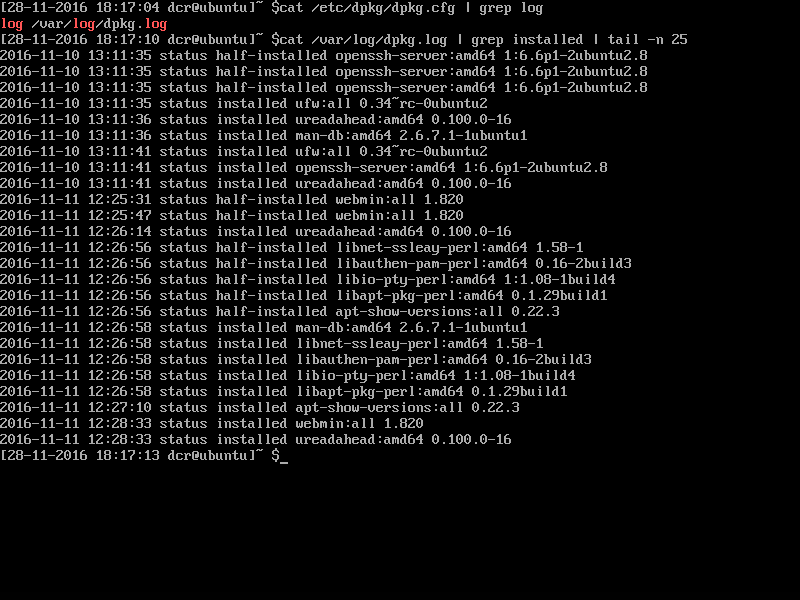
\includegraphics[scale=0.4]{dpkg-log.png}
	\caption{Miramos la localización de log de dpkg en Ubuntu Server y miramos las últimas 25 líneas que contienen \textit{installed}.}
\end{figure}

En CentOS utilizamos \textit{yum (Yellowdog Updater Modified)} por lo que hemos de mirar en el parámetro logfile de su archivo de configuración \cite{c1a3} para saber su ubicación, que resulta ser \verb|/var/log/yum.log| como podemos apreciar en la figura.
\begin{figure}[H]
	\centering
	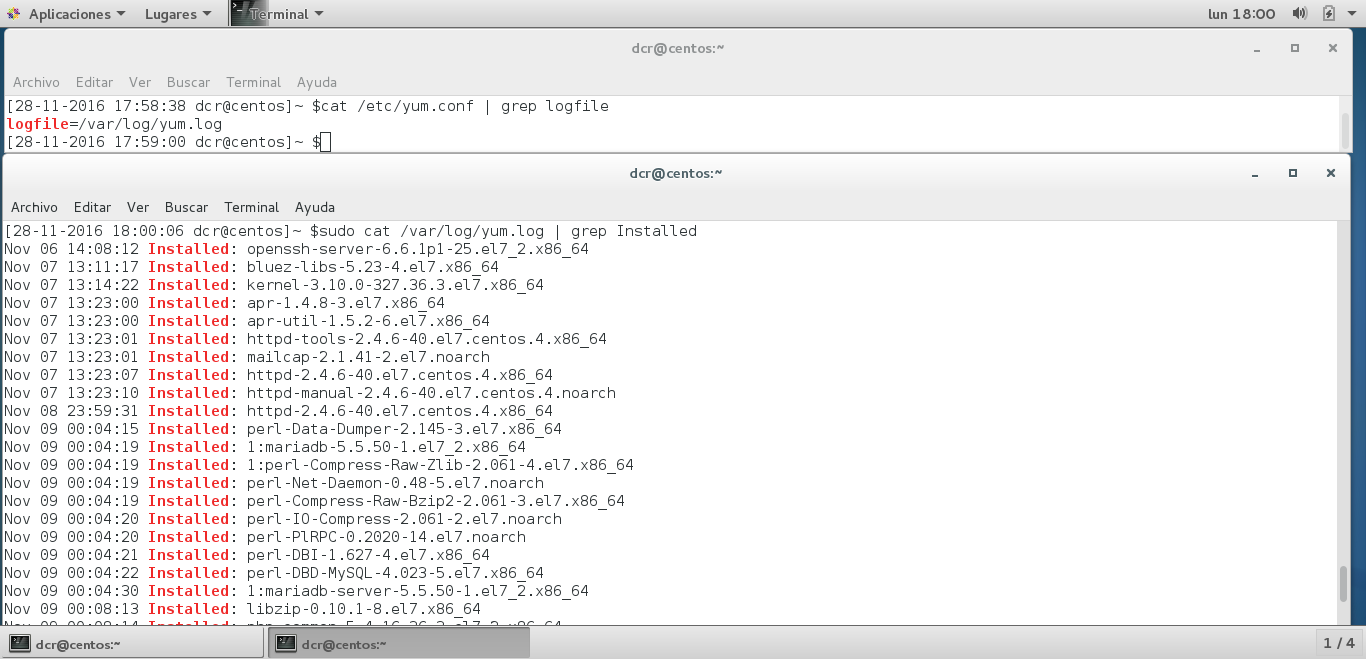
\includegraphics[scale=0.4]{yum-log.png}
	\caption{Miramos la localización de log de yum en CentOS y miramos las líneas que contienen \textit{Installed}.}
\end{figure}

\textit{Nota: Tanto para yum como para dpkg, aunque estemos viendo una lista y \linebreak seleccionando los instalados, que un programa se encuentre en dicha lista \linebreak no implica que en el momento actual se encuentren instalados en el sistema, sino que en algún momento el gestor de paquetes realizó su instalación.}
\linebreak\linebreak
Las terminaciones \verb|*.gz| en el directorio \verb|/var/log/| indican que son antiguas versiones del \textit{log} comprimidas con \textit{gzip} debido a la utilidad \textbf{\textit{logrotate}} \cite{c1b} normalmente. Dicha utilidad nos permite periódicamente (según queramos configurarlo) rotar, comprimir y eliminar tras un cierto número de rotaciones un log antiguo. En Ubuntu Server 14.04 podemos observar el log \textit{dmesg}.

\begin{figure}[H]
	\centering
	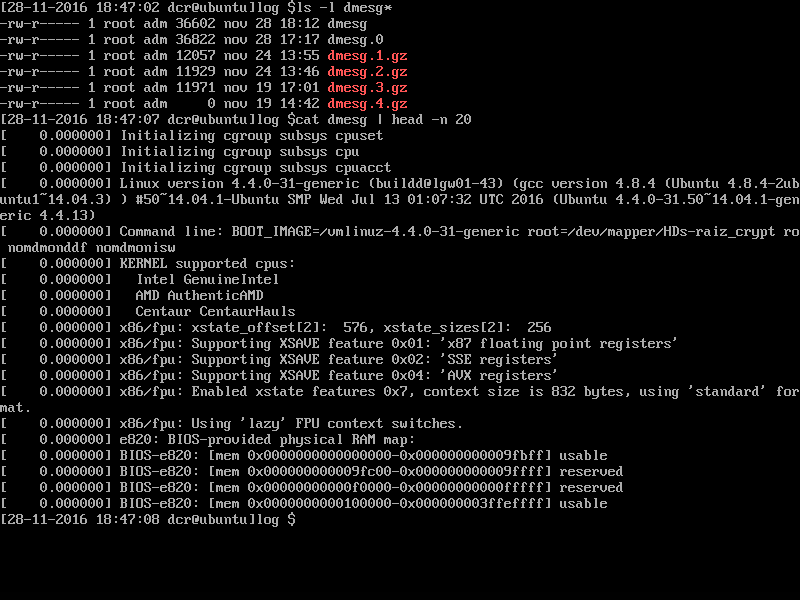
\includegraphics[scale=0.4]{dmesg.png}
	\caption{Miramos las fechas de los archivos que empiezan con dmesg en /var/log y las primeras 20 líneas del último dmesg.}
\end{figure}

Podemos observar que las rotaciones más antiguas son las que van adquiriendo un número mayor y que sólo se guardan rotaciones de la 0 a la 4 así como la actual.
Probemos que efectivamente son archivos comprimidos con gzip y comparémoslo con el log actual.

\begin{figure}[H]
	\centering
	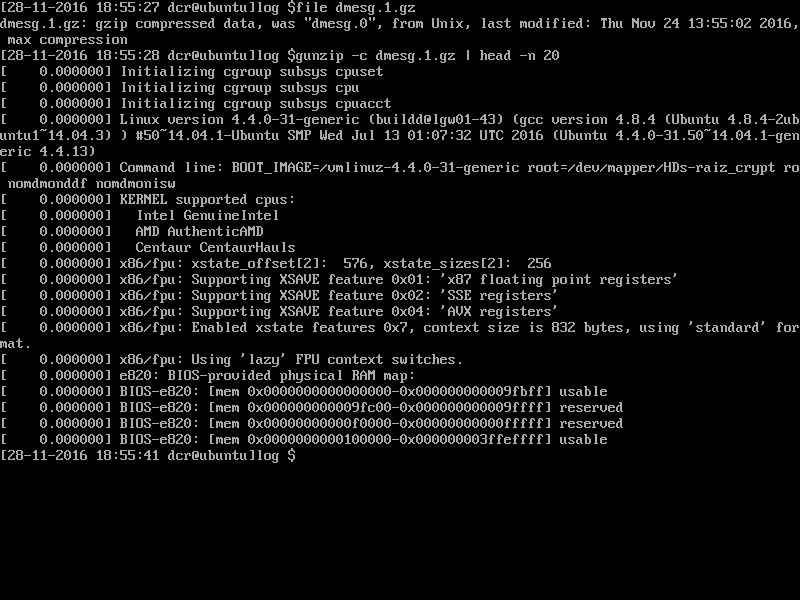
\includegraphics[scale=0.4]{dmesg1.png}
	\caption{Comprobamos el tipo de archivo con \textit{file\cite{c1b2}} y utilizamos \textit{gunzip -c\cite{c1b3}} para mostrar su contenido.}
\end{figure}

Podemos observar que el contenido de ambas para las primeras líneas es el mismo ya que corresponde a contenido escrito por el kernel al arrancar, probemos ahora con las últimas líneas.

\begin{figure}[H]
	\centering
	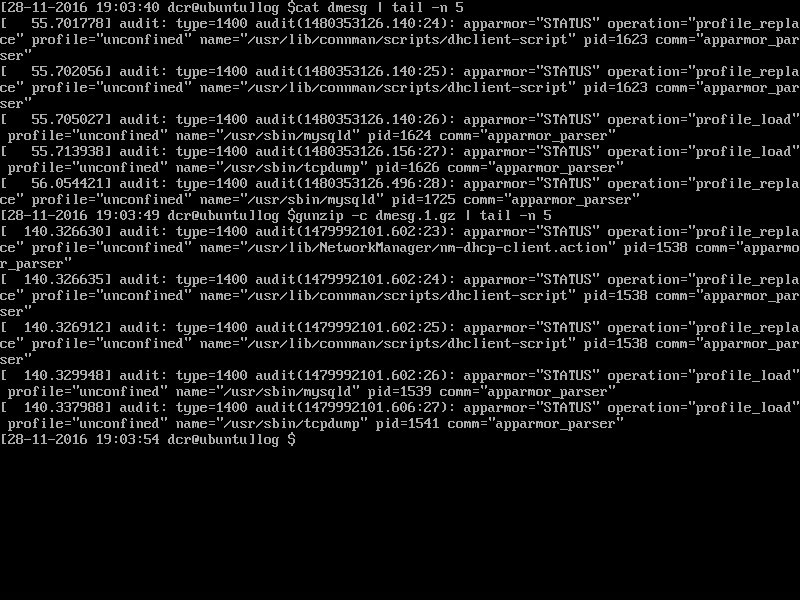
\includegraphics[scale=0.4]{dmesg2.png}
	\caption{Comprobamos ahora las últimas lineas del archivo.}
\end{figure}

Aunque los mensajes son bastante parecidos podemos observar que hay diferencias en la marca de tiempo puesta desde que el sistema había arrancado en cada uno de los casos. 



%----------------------------------------------------------------------------------------
%	Cuestión 2
%----------------------------------------------------------------------------------------
\section{¿Qué archivo ha de modificar para programar una tarea? Escriba la línea necesaria para ejecutar una vez al día una copia del directorio \~/codigo a \~/seguridad/\$fecha donde \$fecha es la fecha actual (puede usar el comando date).}

\subsection{Ubuntu Server 14.04}
En Ubuntu el archivo a modificar para programar una tarea es /var/spool/cron/crontabs/\$user (donde \$user es el nombre del usuario que quiere añadir el trabajo de cron) \cite{c2a}.

Para añadir la tarea diaria editamos dicho archivo. Para ello podemos utilizar \verb|crontab -e|\cite{c2a1} al editarlo añadimos la siguiente línea:\linebreak
\begin{verbatim}
0 13 * * * mkdir ~/"seguridad/$(date +\%d-\%m-\%Y)" && cp -R ~/codigo 
~/"seguridad/$(date +\%d-\%m-\%Y)"
\end{verbatim}

\textit{Nota: He puesto 13 como hora para poder comprobar rápidamente que funciona correctamente. Lo más habitual es ponerlo a las 12 de la noche (0) o a alguna otra hora con poca carga de trabajo (relativa) para el servidor.}
\linebreak\linebreak

Antes de comprobar el funcionamiento correcto de \textit{crontab} vamos a comprobar que efectivamente con \verb|crontab -e| hemos modificado el archivo que se nos ha indicado realizado un \textit{cat} sobre el mismo, tal y como podemos apreciar en la siguiente captura de pantalla.

\begin{figure}[H]
	\centering
	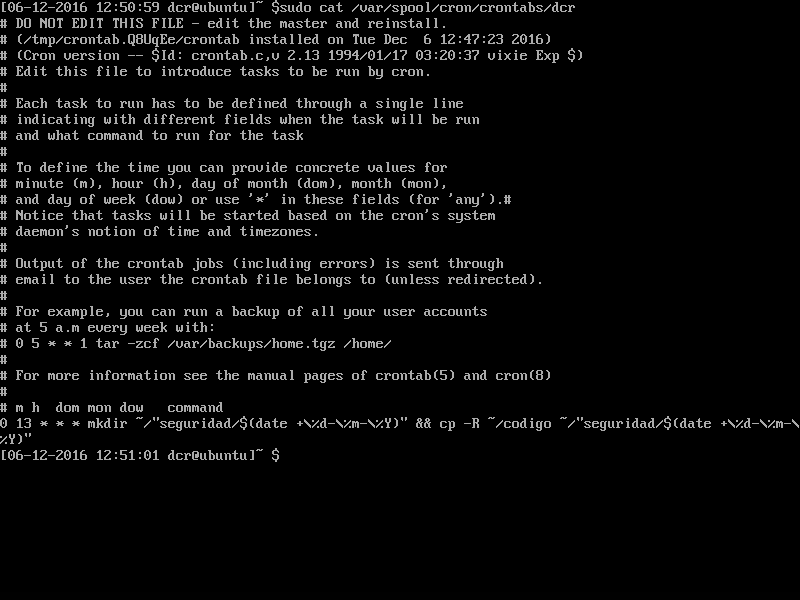
\includegraphics[scale=0.4]{cron-ubuLocation.png}
	\caption{Comprobamos con cat que hemos modificado el archivo indicado en la documentación.}
\end{figure}

Al llegar la hora vamos a comprobar que efectivamente se ha ejecutado la tarea. Primero miramos el log del sistema para ver si efectivamente se ha ejecutado la orden indicada y luego revisaremos que efectivamente ha aparecido una nueva carpeta con la fecha del día y se ha creado a las 13:00.

\begin{figure}[H]
	\centering
	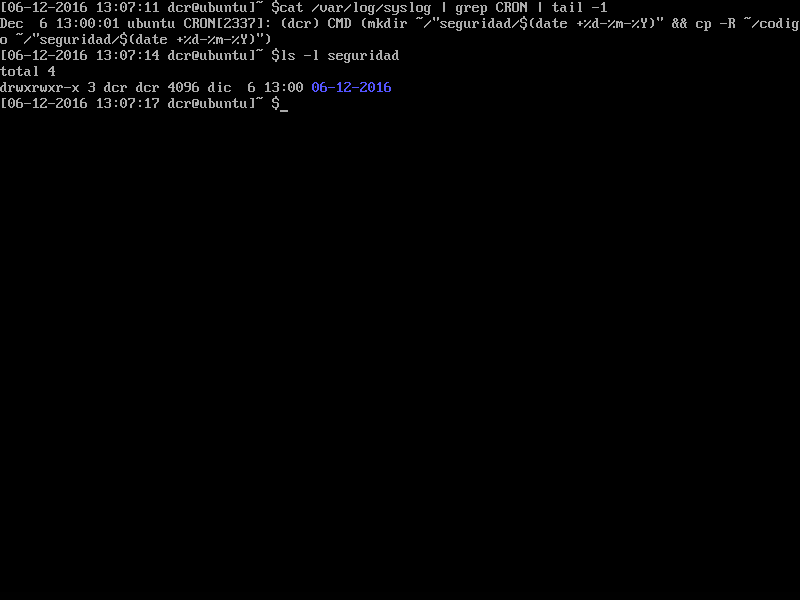
\includegraphics[scale=0.4]{cron-ubuCheck.png}
	\caption{Comprobamos que efectivamente se ha ejecutado la tarea de cron.}
\end{figure}


\subsection{CentOS}
En CentOS el archivo a modificar para programar una tarea es /var/spool/cron/\$user (donde \$user es el nombre del usuario que quiere añadir el trabajo de cron) \cite{c2b}.
%----------------------------------------------------------------------------------------
%	Cuestión 3
%----------------------------------------------------------------------------------------
\section{Pruebe a ejecutar el comando, conectar un dispositivo USB y vuelva a ejecutar el comando. Copie y pegue la salida del comando. (considere usar dmesg | tail). Comente qué observa en la información mostrada.}
\begin{figure}[H]
	\centering
	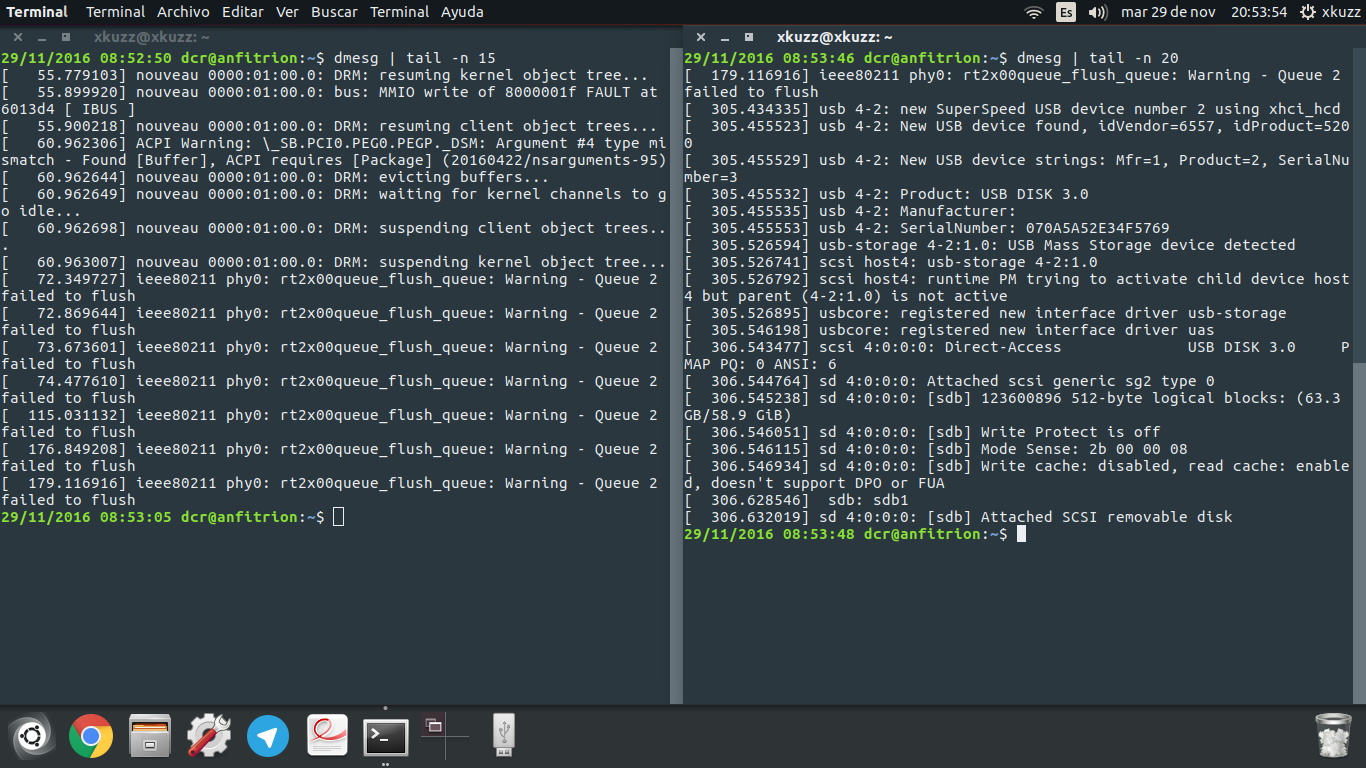
\includegraphics[scale=0.3]{usb.png}
	\caption{A la izquierda \textit{dmesg} sin introducir el dispositivo USB, a la derecha \textit{dmesg} nada más conectarlo.}
\end{figure}

Podemos ver que aparece que se ha conectado un nuevo dispositivo USB, al que se le asocia un número de dispositivo y se nos muestra una serie de detalles como su identificador de producto, identificador de vendedor o el número de serie \cite{c3}. El sistema determina que es una unidad de almacenamiento (\textit{storage}) y la monta en \verb|sdb| mostrando información como el tamaño de bloque lógico (512 bytes) y la capacidad de almacenamiento del dispositivo (58.9 GiB) o si está activado el modo de protección contra escritura.


%----------------------------------------------------------------------------------------
%	Cuestión 4
%----------------------------------------------------------------------------------------
\section{Ejecute el monitor de “System Performance” y muestre el resultado. Incluya capturas de pantalla comentando la información que aparece.}
Tras iniciar el monitor utilizando el comando \verb|perfmon| en una ventana de consola de PowerShell hacemos click en Herramientas de supervisión \textgreater Monitor de Rendimiento y pulsamos en el botón \verb|+| para añadir los parámetros que deseamos observar. En esa ventana agregamos los que nos interese monitorizar y al pulsar sobre ellos si tenemos marcada la casilla \textit{``Mostrar descripción''} podemos información un poco más detallada sobre lo que monitorizan. \cite{c4}
\begin{figure}[H]
	\centering
	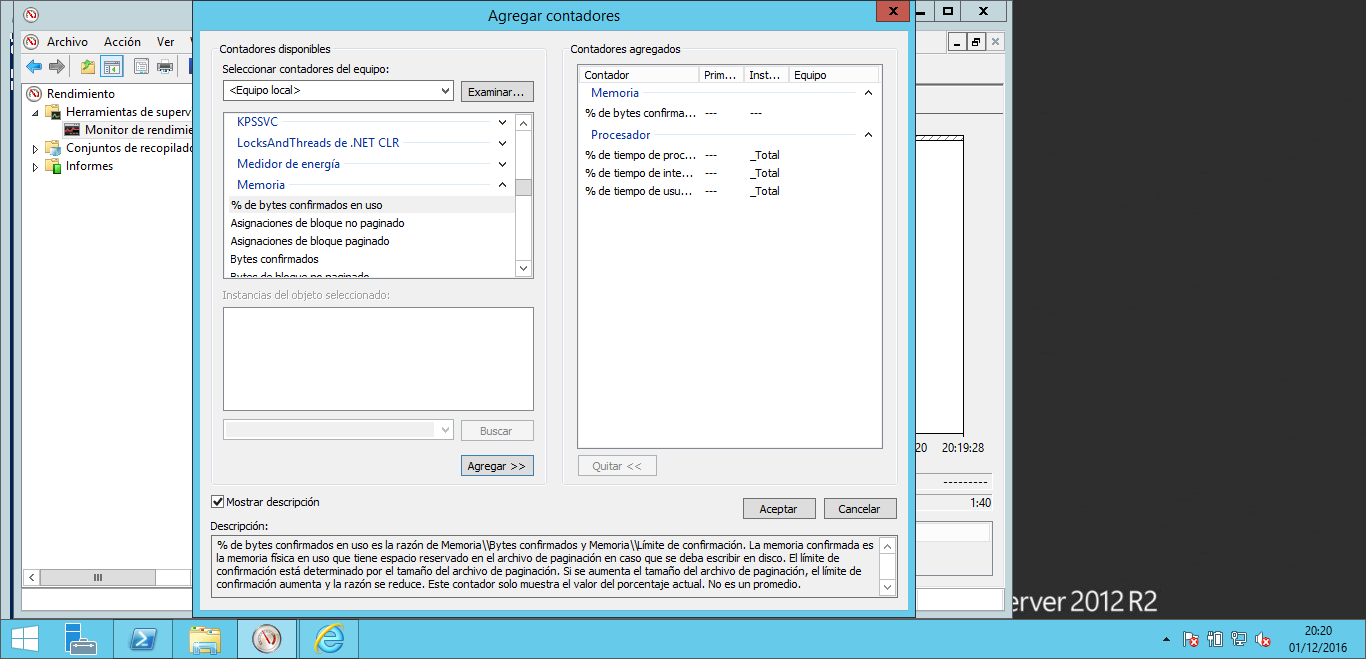
\includegraphics[scale=0.4]{perfmonContadores.png}
	\caption{Ventana en la que seleccionamos los elementos que vamos a monitorizar.}
\end{figure}

Vamos a analizar el comportamiento del sistema mientras usamos la máquina para realizar las siguientes cosas: iniciar la descarga de un archivo grande para que no termine la descarga durante el tiempo de monitorización, en plena descarga cargamos una página con gran cantidad de contenido multimedia (YouTube) posteriormente cerramos la página con contenido multimedia y por último cancelamos la descarga.

\begin{itemize}
  \item \textbf{\% tiempo de procesador} \textit{(Línea verde)} - Porcentaje de tiempo que el procesador se encuentra atendiendo algún proceso activo (Existe un proceso inactivo que consume ciclos cuando no hay procesos activos listos para usar el procesador).
  \item \textbf{\% tiempo de usuario} \textit{(Línea amarilla)} - Porcentaje de tiempo que el procesador se encuentra trabajando en modo usuario. (Existe también el modo privilegiado que es utilizado exclusivamente por el sistema operativo y las llamadas que se hacen al mismo).
  \item \textbf{\% tiempo de interrupciones} \textit{(Línea azul)} - Porcentaje de tiempo que el procesador se encuentra atendiendo interrupciones hardware.
  \item \textbf{\% de bytes confirmados en memoria} \textit{(Línea roja)} - Memoria física en uso que tiene espacio reservado en el archivo de paginación si hubiese que guardar memoria en disco.
\end{itemize}

\begin{figure}[H]
	\centering
	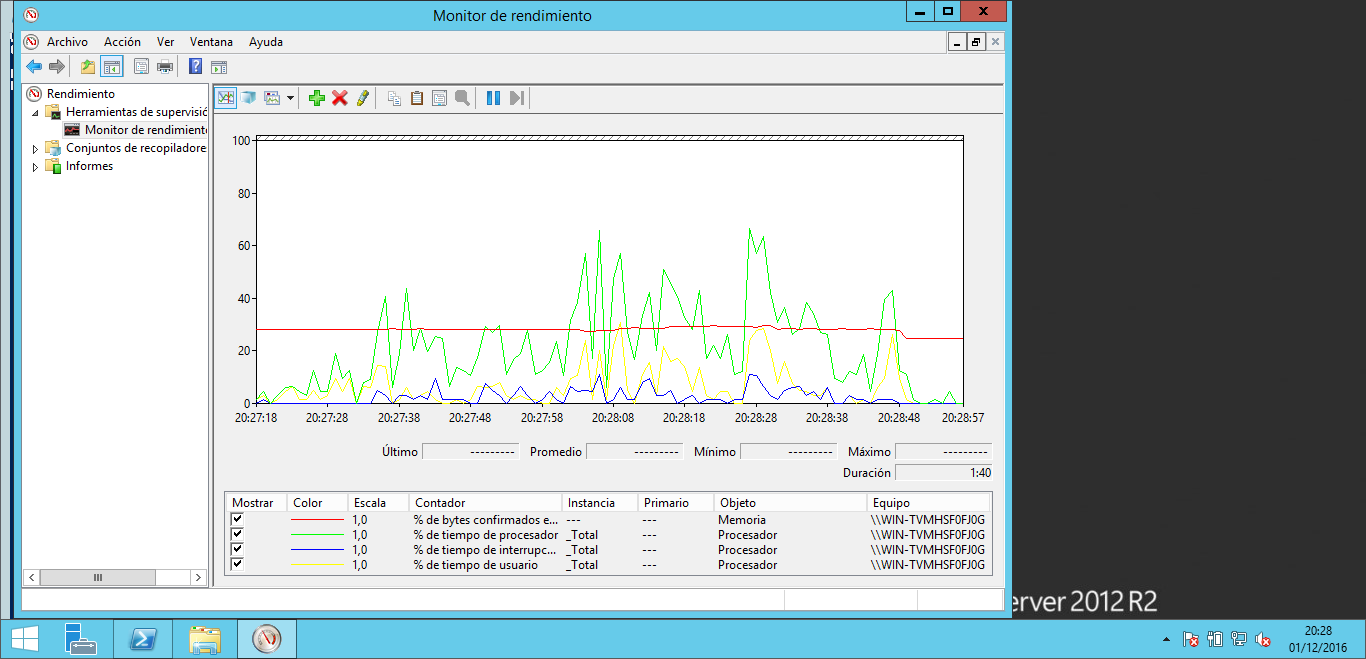
\includegraphics[scale=0.4]{perfmon.png}
	\caption{Gráfico de la monitorización en Windows Server 2012 R2 de los parámetros propuestos.}
\end{figure}

Al inicio nos encontramos navegando para buscar el archivo a descargar, por lo que vemos que del porcentaje de uso del procesador la mayor parte es en modo usuario. Una vez se inicia la descarga y hasta que se cancela podemos observar pequeños picos en el porcentaje de tiempo que se encuentra atendiendo interrupciones hardware. Estas deben ser interrupciones de disco provocadas por la descarga. Justo en el centro de la gráfica vemos los mayores picos en el uso de la CPU, en ese momento nos encontramos abriendo un vídeo en YouTube mientras sigue la descarga y dentro de esos picos vemos que hay gran parte de llamadas al sistema por la diferencia que existe entre el porcentaje de tiempo de procesador y el porcentaje de tiempo de procesador en modo usuario. Conforme se van cancelando y cerrando las pestañas del navegador podemos apreciar como rápidamente los porcentajes de procesador, procesador atendiendo interrupciones y procesador en modo usuario	bajan a valores muy cercanos al 0 \%. Por último, nos queda hablar del porcentaje de bytes confirmados en memoria, puesto que las operaciones que han realizado no han necesitado de grandes cantidades de memoria sólo vemos ligeros cambios en el mismo.


%----------------------------------------------------------------------------------------
%	Cuestión 5
%----------------------------------------------------------------------------------------
\section{Cree un recopilador de datos definido por el usuario (modo avanzado) que incluya tanto el contador de rendimiento como los datos de seguimiento. Almacene el resultado en el directorio \textit{Escritorio\textbackslash logs}. Incluya las capturas de pantalla de cada paso.}
Para empezar tal y como hicimos en la cuestión anterior abrimos una consola de PowerShell y utilizamos el comando \verb|perfmon|. Tras abrirse la ventana del monitor del rendimiento en el menú lateral abrimos la pestaña \textit{Conjunto de recopiladores de datos} y haciendo click derecho en \textit{Definido por el usuario} pinchamos en \textit{Nuevo \textgreater Conjunto de recopiladores de datos} y seguimos los pasos indicados en las capturas de pantalla siguientes para configurarlo. \cite{c5}
\begin{figure}[H]
	\centering
	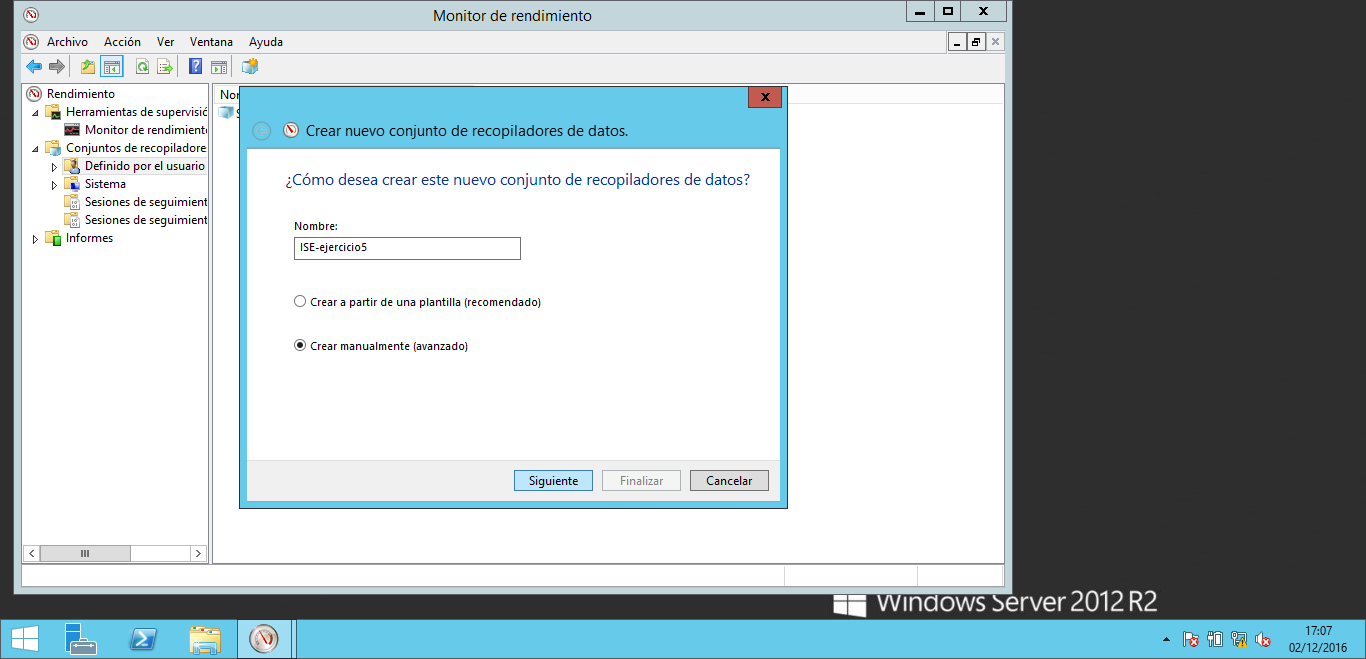
\includegraphics[scale=0.4]{recopilador-1.png}
	\caption{Le damos un nombre al recopilador de datos (en mi caso, ISE-ejercicio5) y marcamos \textit{Crear manualmente (avanzado)} antes de pulsar \textit{Siguiente}.}
\end{figure}

\begin{figure}[H]
	\centering
	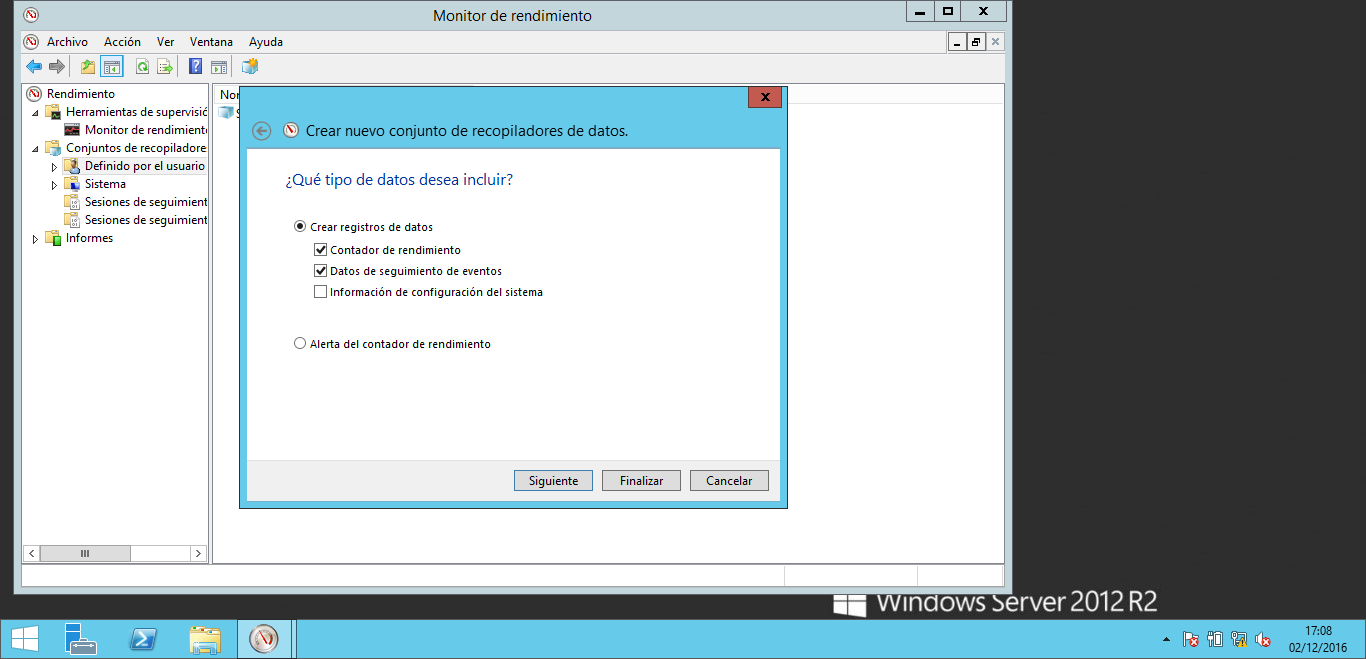
\includegraphics[scale=0.4]{recopilador-2.png}
	\caption{Dejamos \textit{Crear registro de datos}, marcamos \textit{Contador de rendimiento} y \textit{Datos de seguimiento de eventos} y pulsamos en \textit{Siguiente}.}
\end{figure}

\begin{figure}[H]
	\centering
	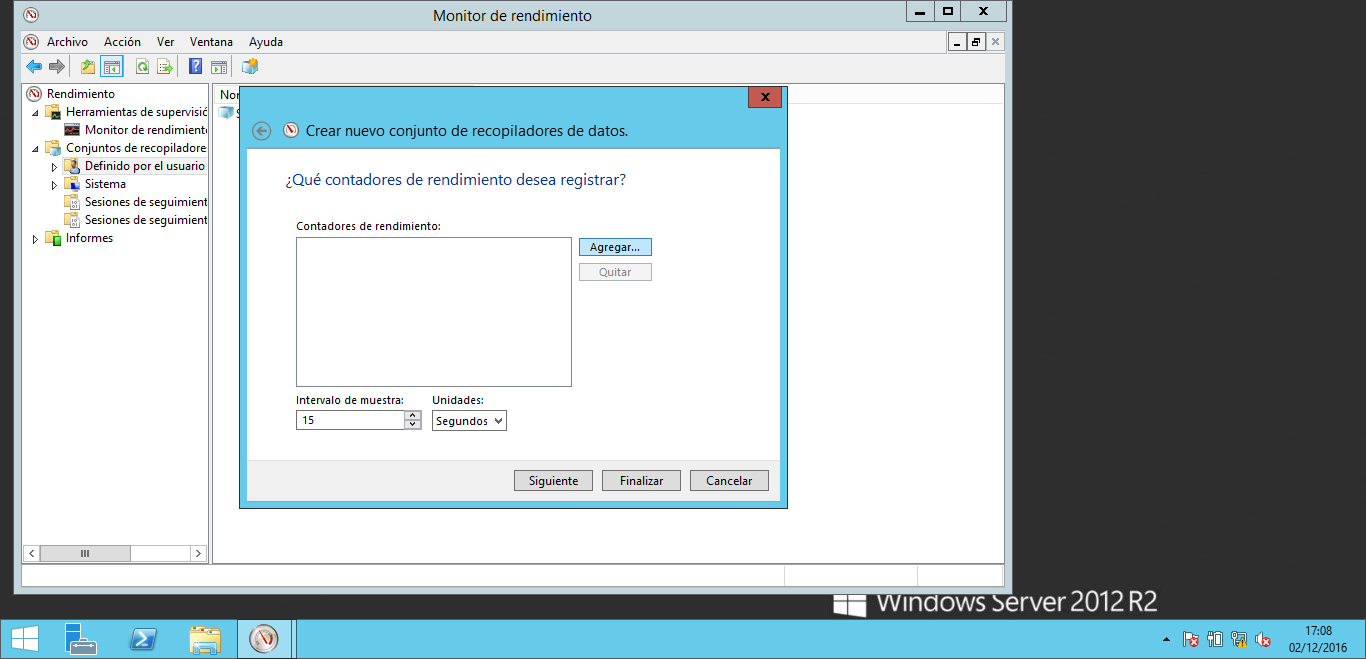
\includegraphics[scale=0.4]{recopilador-3.png}
	\caption{Dejamos el intervalo de muestra en 15 segundos y pulsamos en \textit{Agregar...}.}
\end{figure}

\begin{figure}[H]
	\centering
	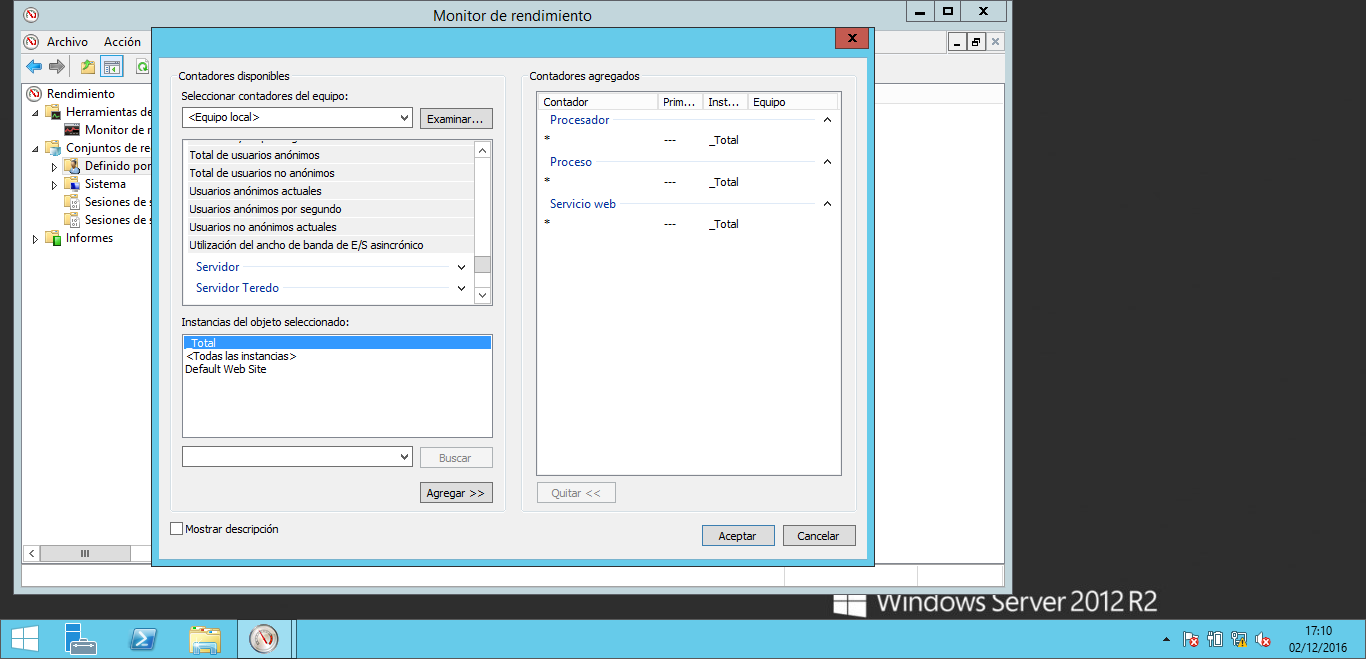
\includegraphics[scale=0.4]{recopilador-4.png}
	\caption{Seleccionamos todos los campos relativos a las secciones \textit{Procesador}, \textit{Proceso} y \textit{Servicio web}. }
\end{figure}

\textit{Nota: Podemos añadir todos los campos de una sección pulsando el primero y mientras pulsamos la teclas ``Mayus'' pulsamos el último, seleccionando todo el rango de valores y añadiéndolos pulsando en Agregar \textgreater \textgreater.}

\begin{figure}[H]
	\centering
	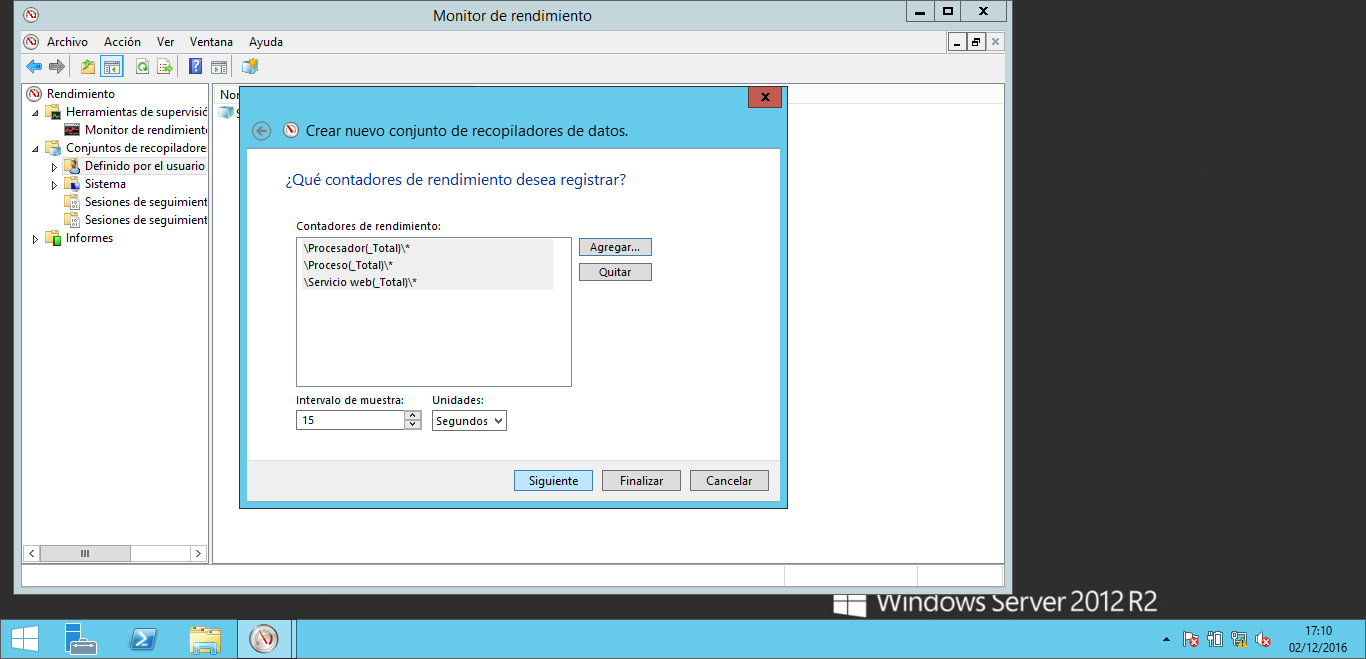
\includegraphics[scale=0.4]{recopilador-5.png}
	\caption{Revisamos que efectivamente se han añadido todos los campos de las tres áreas mencionadas (indicando con un * para cada área) y pulsamos en \textit{Siguiente}.}
\end{figure}

\begin{figure}[H]
	\centering
	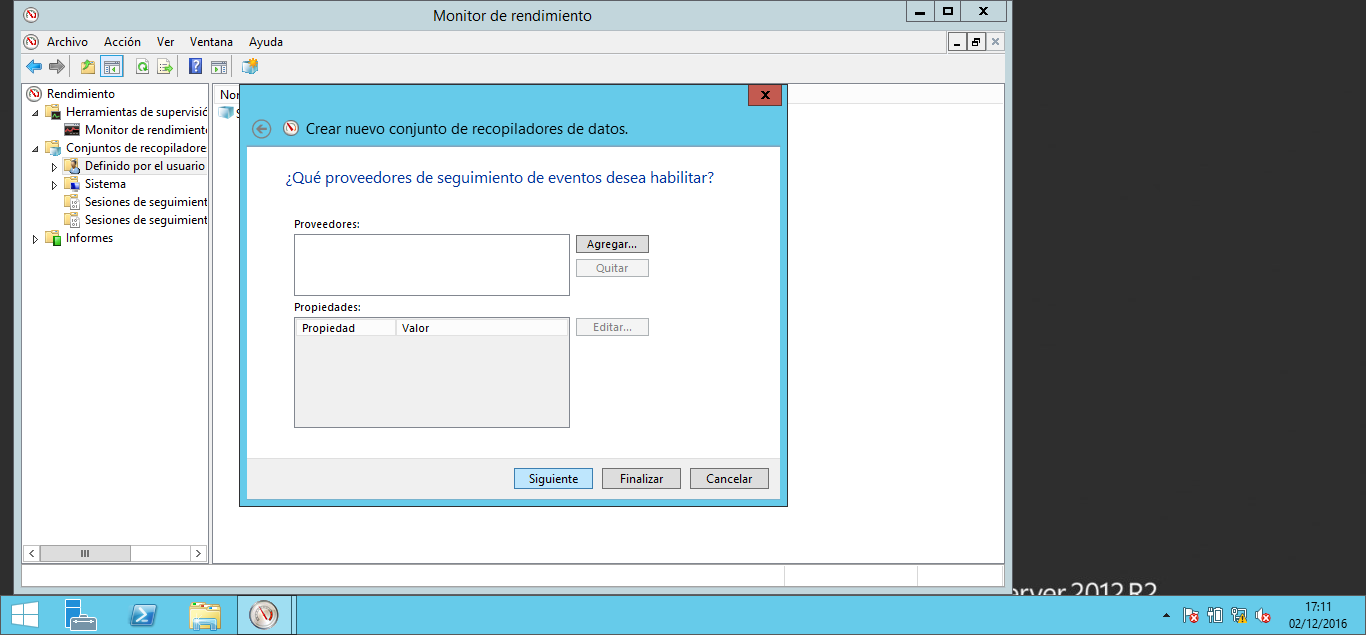
\includegraphics[scale=0.4]{recopilador-6.png}
	\caption{Volvemos a pulsar en \textit{Siguiente}.}
\end{figure}

\begin{figure}[H]
	\centering
	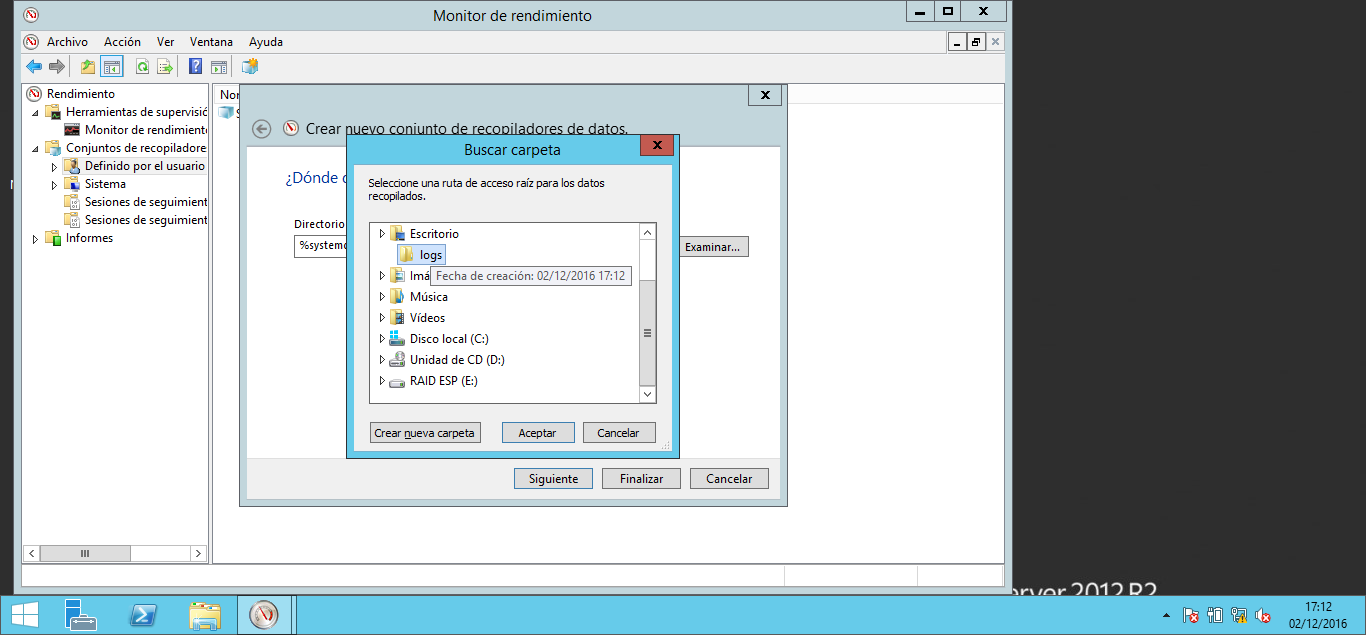
\includegraphics[scale=0.4]{recopilador-7.png}
	\caption{Pulsamos en Examinar y seleccionamos la ruta (en mi caso, \protect\url{C:\ Users\ Administrador\ Desktop\ logs}) donde deseamos que se guarden los \textit{logs} del recopilador de datos.}
\end{figure}

\begin{figure}[H]
	\centering
	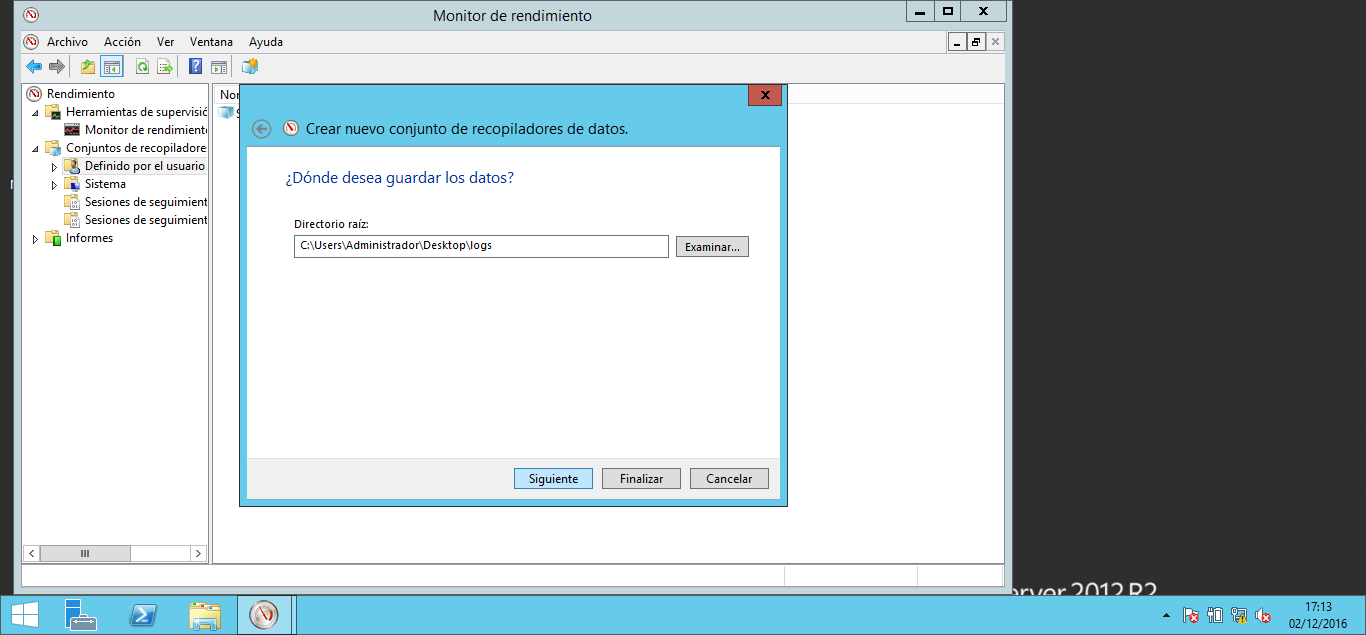
\includegraphics[scale=0.4]{recopilador-8.png}
	\caption{Revisamos que la ruta sea correcta y pulsamos en \textit{Siguiente}.}
\end{figure}

\begin{figure}[H]
	\centering
	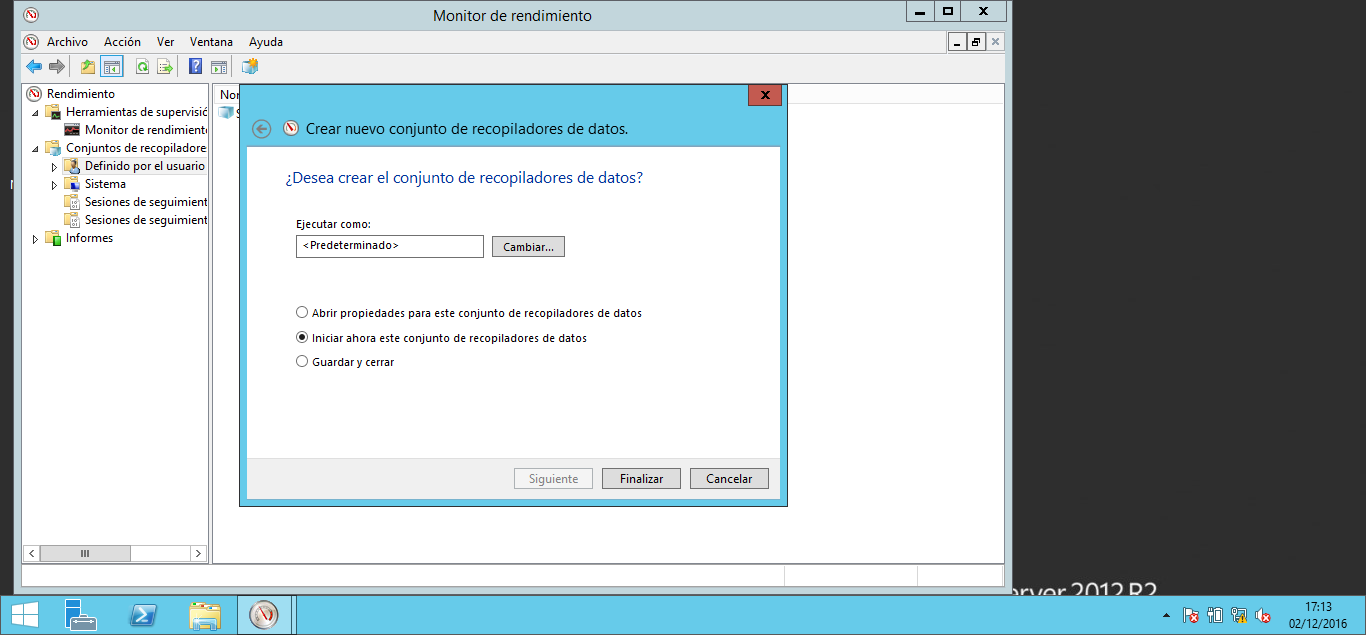
\includegraphics[scale=0.4]{recopilador-9.png}
	\caption{Marcamos \textit{Iniciar ahora este conjunto de recopiladores de datos} (puesto que voy a realizar la monitorización de inmediato) y pulsamos \textit{Finalizar}.}
\end{figure}

\begin{figure}[H]
	\centering
	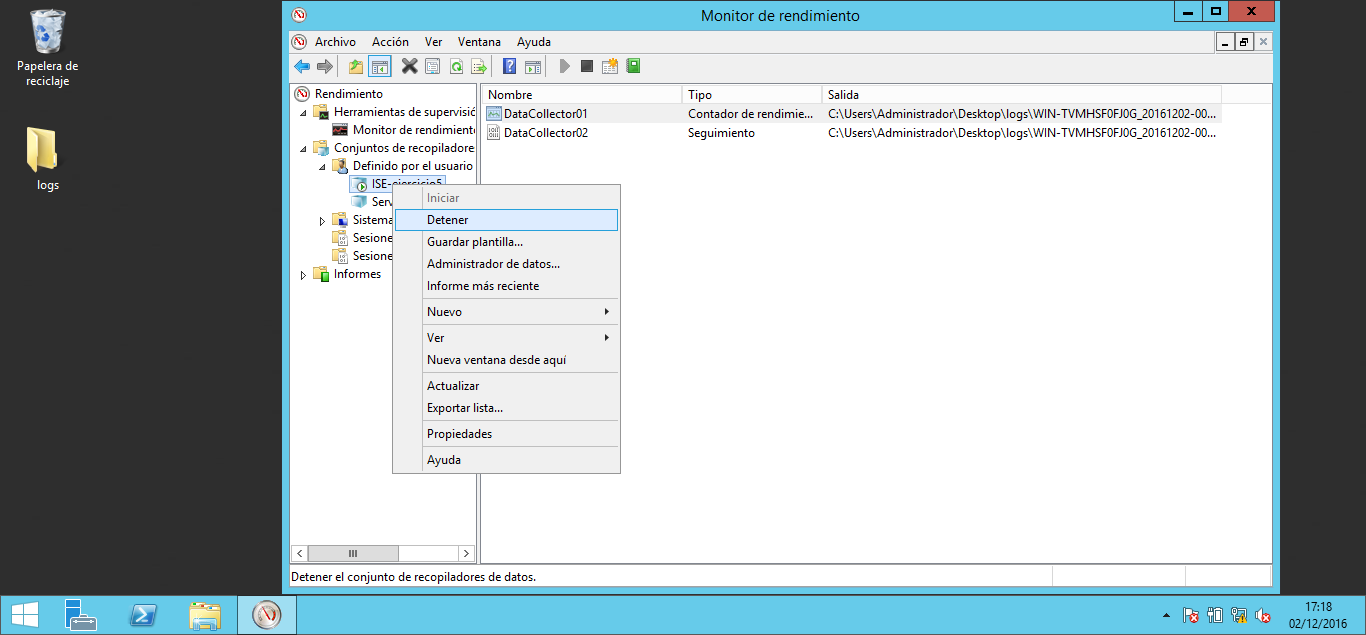
\includegraphics[scale=0.4]{recopilador-10.png}
	\caption{Paramos el recopilador de datos una vez que han pasado 5 minutos haciendo click derecho en el menú lateral al recopilador de datos que tiene el nombre que hemos puesto y pulsamos \textit{Detener}.}
\end{figure}

Tras detenerlo cerramos la ventana y en la ruta en la que hemos almacenado los \textit{logs} encontramos un archivo del monitor del rendimiento. Haciendo doble click en él (en mi caso, nombrado \textit{DataCollector01}) se nos habré una nueva ventana del monitor de rendimiento con la gráfica de lo que ha ocurrido durante el tiempo de monitorización con los parámetros que hemos ido recopilando, tal y como podemos apreciar en la siguiente figura.
\begin{figure}[H]
	\centering
	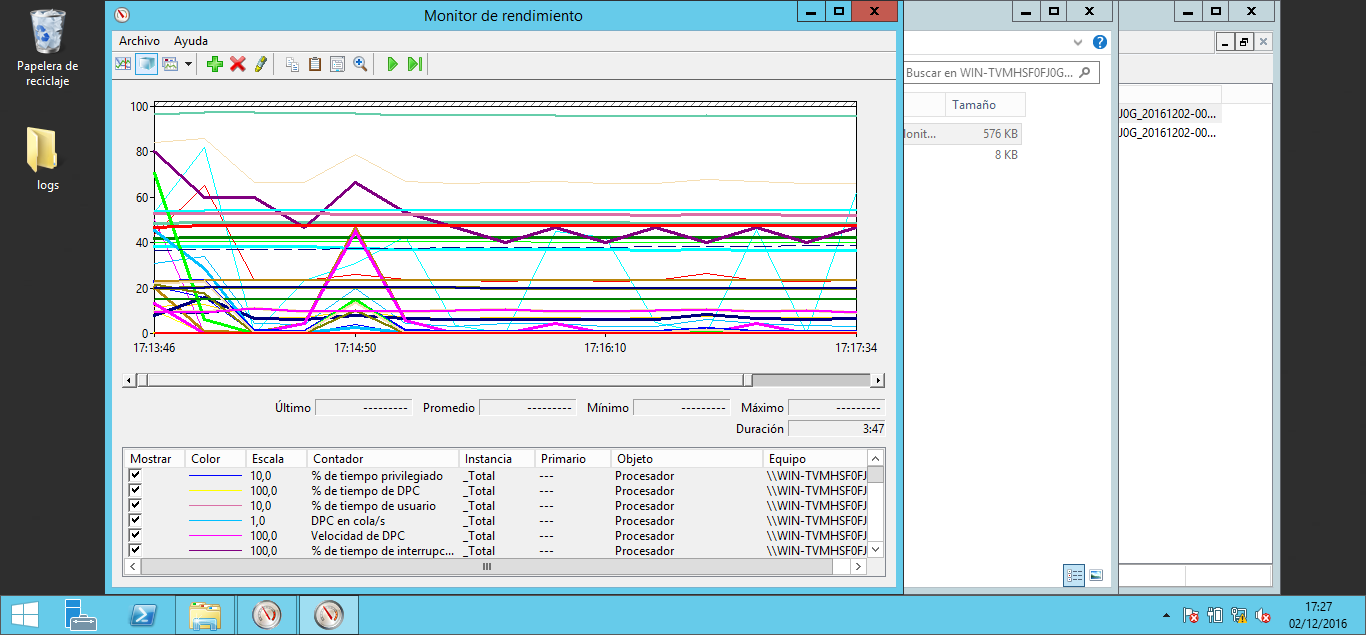
\includegraphics[scale=0.4]{recopilador-completo.png}
	\caption{Gráfica del recopilador de datos mostrando todos los parámetros.}
\end{figure}

Para poder interpretar que es lo que ha ocurrido vamos a seleccionar algunos parámetros de los almacenados, en concreto, vamos a fijarnos en los siguientes:
\begin{itemize}
  \item \textbf{Operaciones ES (Entrada/Salida) de escritura} \textit{(Línea morada gruesa)}.
  \item \textbf{Bytes de escritura de ES} \textit{(Línea rosa)}.
  \item \textbf{Interrupciones} \textit{(Línea amarilla)}
  \item \textbf{Porcentaje de tiempo que el procesador se encuentra activo} \textit{(Línea azul)}.
  \item \textbf{Porcentaje de tiempo que el procesador está atendiendo interrupciones hardware} \textit{(Línea morada fina)}
  \item \textbf{Porcentaje de tiempo del procesador en modo usuario} \textit{(Línea verde)}.
\end{itemize}

\begin{figure}[H]
	\centering
	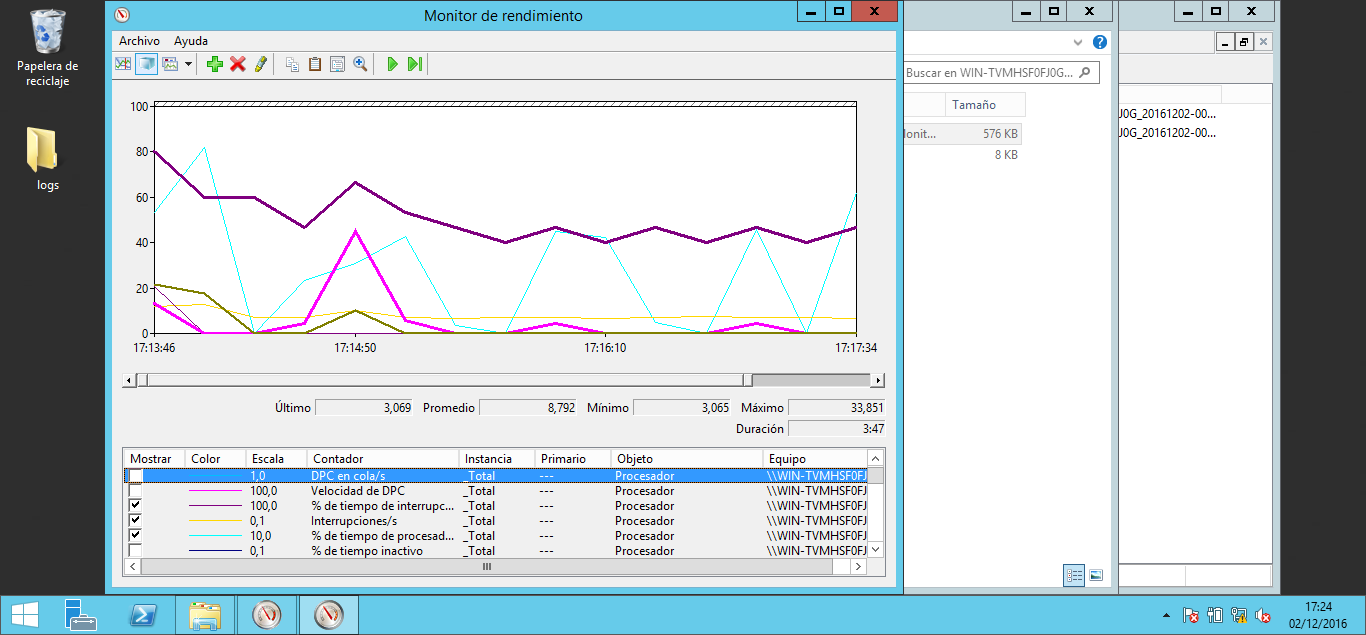
\includegraphics[scale=0.4]{recopilador-seleccion.png}
	\caption{Gráfica del recopilador de datos con una selección de parámetros.}
\end{figure}

Durante los minutos que el recopilador estuvo tomando datos, una vez que revisé que la carpeta de logs se encontraba en su sitio y se estaba guardando algún dato, me puse a utilizar la máquina anfitriona para terminar de explicar la cuestión anterior. \linebreak

En la gráfica podemos apreciar los primeros 3 minutos y 48 segundos. Podemos observar que hay un uso bajo del procesador en modo usuario (probablemente mientras estoy comprobando que el directorio existe y que se ha escrito algo) y luego no es usado (mientras me encuentro en la máquina anfitriona redactando la cuestión anterior). Las operaciones de escritura son altas cuando se inicia el monitor pero vemos que al final se va estabilizando probablemente y se deben a la escritura del log del monitor. También llama la atención el hecho de que a las 17:14:50 se encuentra el máximo absoluto en la gráfica con respecto a ambas medidas de escritura y luego ambas se acaban estabilizando, es posible que se estuviese creando por primera vez el archivo de log y se tuviese que guardar más información de la habitual. Podemos ver que el número de interrupciones hardware es bastante estable y excepto al principio el porcentaje de tiempo que el procesador dedica a dichas interrupciones es prácticamente inapreciable. Por último, observamos la línea de tiempo que el procesador está activo, puesto que no estamos usando la máquina virtual hemos de suponer o que los picos en éste se deben al \textit{overhead} que produce la recopilación de todos estos datos o al uso de la máquina anfitriona.



%----------------------------------------------------------------------------------------
%	Cuestión 6
%----------------------------------------------------------------------------------------
\section{Visite la web del proyecto y acceda a la demo que proporcionan (http://demo.munin-monitoring.org/) donde se muestra cómo monitorizan un servidor. Monitorice varios parámetros y haga capturas de pantalla de lo que está mostrando comentando qué observa.}

Tras entrar en la página web encontramos los siguiente:
\begin{figure}[H]
	\centering
	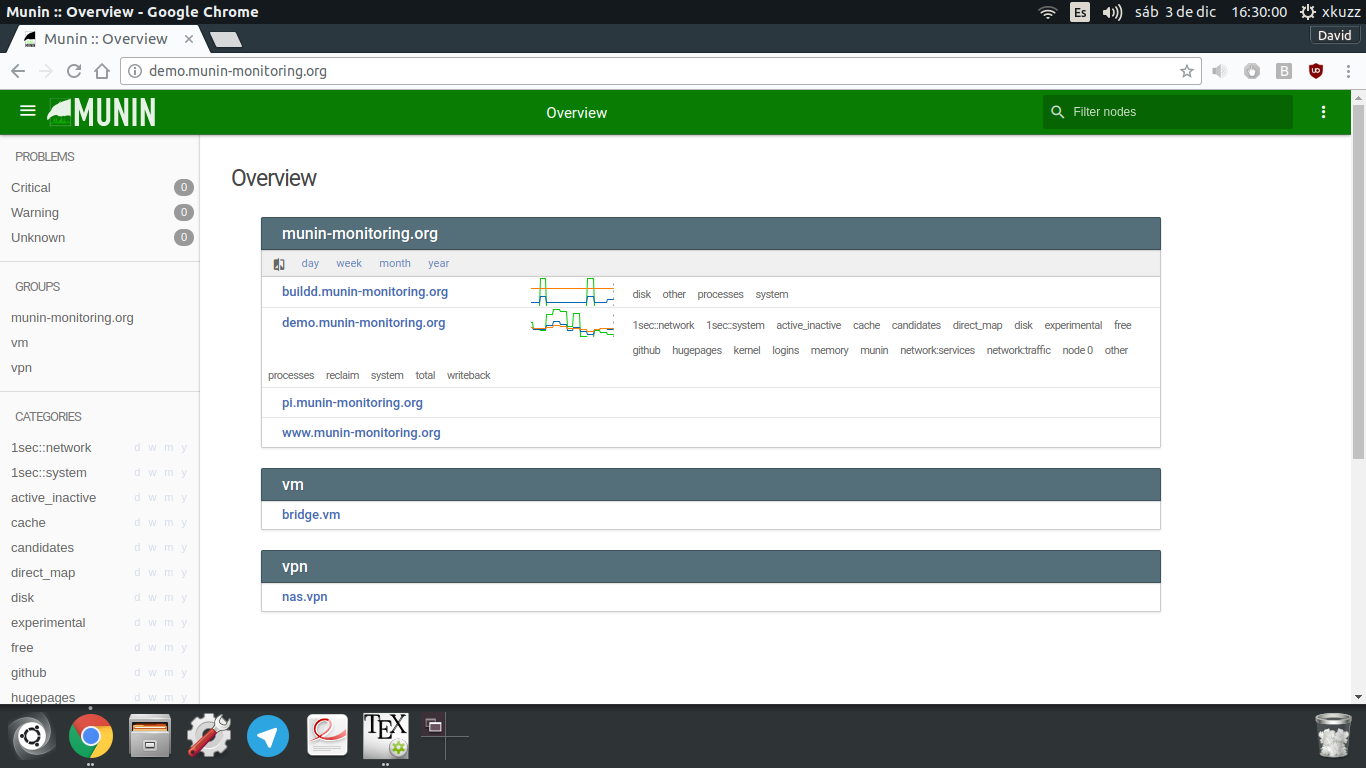
\includegraphics[scale=0.3]{munin1.png}
	\caption{Página de inicio de la demo de munin.}
\end{figure}

A la izquierda podemos un panel en el que se nos informan de posibles prooblemas, disponemos de un filtro para los nodos en el menú superior y en el centro de la imagen tenemos una serie de grupos, de los cuales sólo el primero de ellos contiene algo de información. Primero vamos a visitar la información del sitio \url{buildd.munin-monitoring.org} pulsando en el mismo. Si pulsamos en la parte superior en la pestaña \textit{processes} podemos observar información relativa a los procesos relacionados con ese sitio. 
\begin{figure}[H]
	\centering
	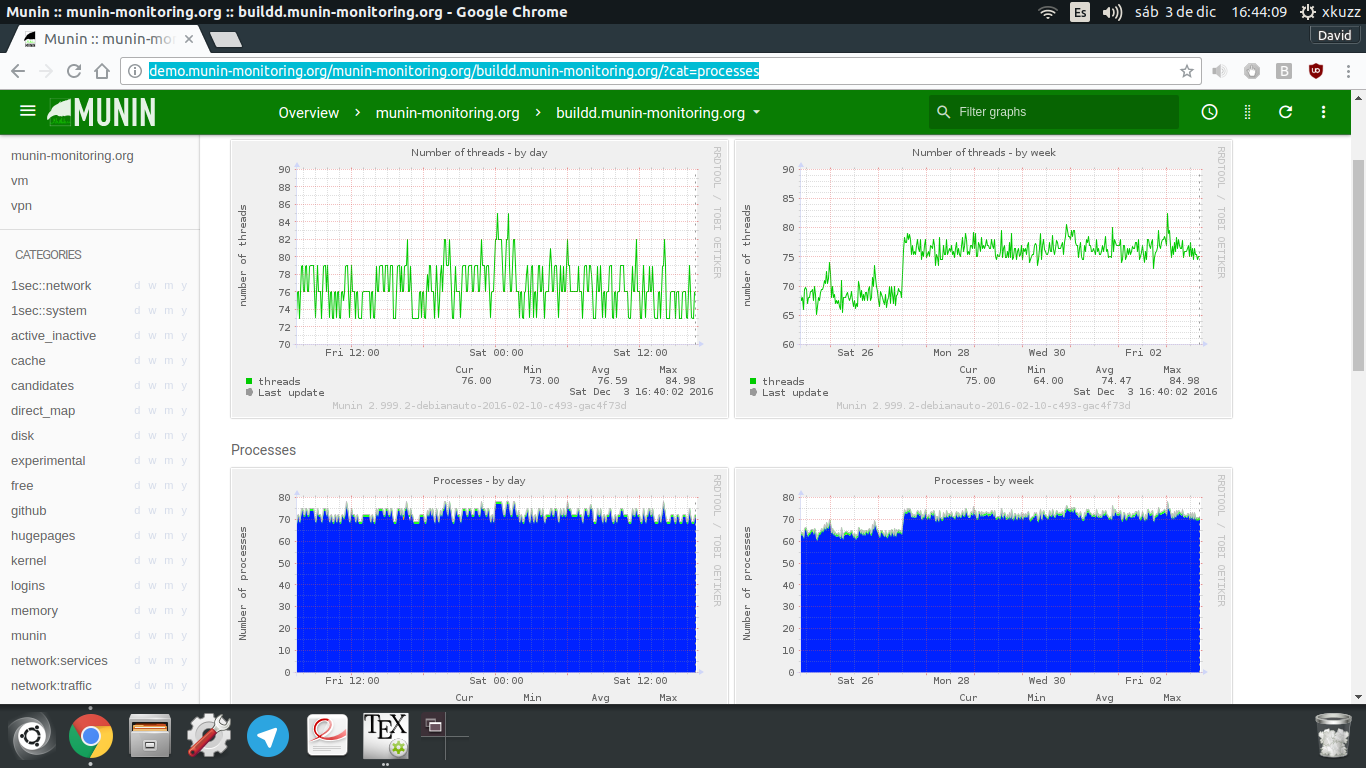
\includegraphics[scale=0.3]{munin2.png}
	\caption{Monitorización de procesos en Munin.}
\end{figure}

Podemos observar como mientras que existen mayores diferencias entre número de hebras que las ligeras diferencias que hay en número de procesos. Y que hay una diferencia considerable de carga del sitio durante el fin de semana anterior con respecto a los días laborables.\linebreak\linebreak

Ahora vamos a pasar a ver un parámetro del otro sitio, para cambiar de sitio pulsamos en el menú que podemos encontrar en la parte superior con el nombre de la url y escogemos el sitio \url{demo.munin-monitoring.org}. En este vamos a seleccionar el disco como parámetro a analizar. Dentro de esta zona encontramos información sobre la latencia de disco, el tiempo de servicio de entrada/salida, el uso del sistema de archivos o el número de operaciones de entrada/salida por segundo, en el que nos vamos a centrar.
\begin{figure}[H]
	\centering
	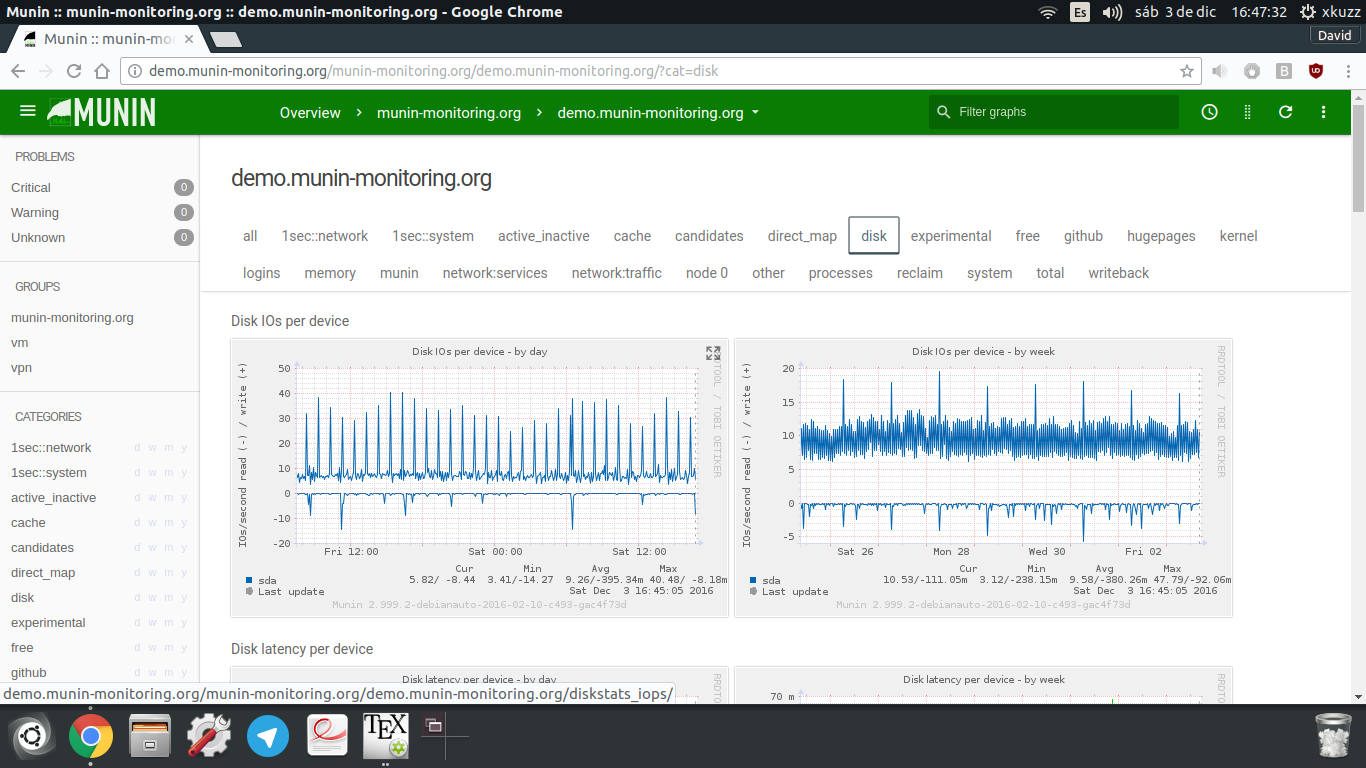
\includegraphics[scale=0.3]{munin3.png}
	\caption{Monitorización de disco en Munin.}
\end{figure}
Podemos observar una serie de periódicas y de similares dimensiones en las escrituras en disco a lo largo de un día (escrituras de log, tareas temporales de 1 o 2 horas) y que son consecuentes también en la semana, aunque parece ser que al inicio de cada día se ejecutan más escrituras (tareas diarias). Las lecturas son más irregulares y las diferencias probablemente se deban al uso humano del sistema en vez de cualquier procedimiento automático. \linebreak\linebreak

Para acabar vamos a mirar otro parámetro más de este mismo sitio así que en la parte superior vamos a seleccionar la pestaña memory. Dentro esta zona podemos gráficas sobre el uso de swap, la fragmentación externa, el uso de memoria virtual y el uso de memoria física en el que nos vamos a centrar.
\begin{figure}[H]
	\centering
	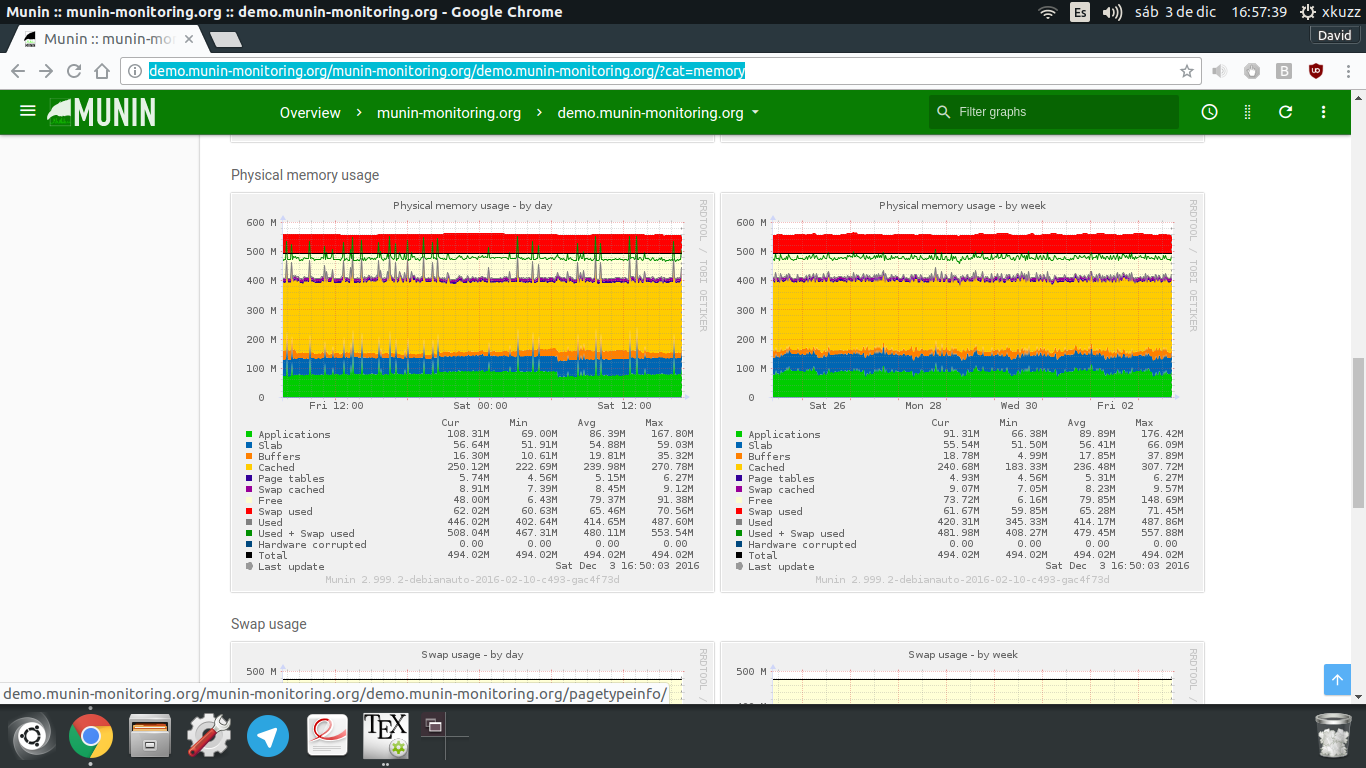
\includegraphics[scale=0.3]{munin4.png}
	\caption{Monitorización de memoria en Munin.}
\end{figure}

Podemos observar que \textit{Munin} nos ofrece una gráfica muy detallada sobre el uso de memoria, podemos observar cuanto memoria se dedica a cosas como aplicaciones, memoria que se encuentra en caché, memoria libre, etc. Vemos que durante el día existe un uso más o menos regular de memoria con algunos picos y que en las horas cercanas a las 0:00 del sábado observamos un intervalo de un menor uso relativo respecto a el resto del intervalo del día monitorizado. En el gráfico semanal podemos observar que apenas hay variaciones significativas en el uso. Es interesante que el uso de memoria en el servidor está limitada a 500 M y normalmente está memoria es utilizada prácticamente por completo todos los días y a diario, indicando que quizás se ha ajustado el funcionamiento del servidor y puesto sólo la cantidad de recursos de memoria justo y necesario para que junto con el swap el sistema funcione correctamente.

%----------------------------------------------------------------------------------------
%	Cuestión 7
%----------------------------------------------------------------------------------------
\section{Escriba un breve resumen sobre alguno de los artículos donde se muestra el uso de strace o busque otro y coméntelo.}
He escogido el segundo artículo propuesto.\cite{c7a} \linebreak\linebreak

Tras indicar el autor que \textit{strace} nos herramienta para depuración ni para programadores sino para administradores de sistemas nos presenta tres casos diferentes en los que podemos usar dicha herramienta. El primero de ellos es un simple ejemplo introductorio en el que se hace \textit{cat} sobre un archivo, al ejecutar \textit{strace} sobre ese ejemplo obtenemos todas las llamadas del sistema asociadas. El autor destaca dos líneas, la línea de \textit{open} que nos indica qué fichero se ha abierto y cómo se ha abierto (lo cual puede resultar más útil para llamadas de las que desconocemos que archivos se van a abrir) y la línea de \textit{read} en la que sólo se muestran los primeros 32 caracteres que se van a leer pero indicando cuantos caracteres se leen en total.\linebreak 

El segundo ejemplo nos ayuda a encontrar archivos de ``logs'' cuando no sabemos dónde se encuentran, para ello reinicia un servicio y hace \textit{strace} sobre todas las bifurcaciones posibles que se creen y guardando la información en un archivo de salida. Tras buscar ``log'' con la herramienta \textit{grep} encuentra las llamadas \textit{open} con las que se habían abierto dichos archivos con sus localizaciones. \linebreak 

Por último, nos enseña un ejemplo en el que detecta un error al iniciar apache tras buscar el código de error que devuelven las llamadas del sistema (-1) con \textit{grep} para delimitar las causas de que apache no arrancase. En ese ejemplo, el log de apache estaba puesto como inmutable y por tanto al realizar \textit{open} con intención de escribir se le denegaba el acceso.


%----------------------------------------------------------------------------------------
%	Cuestión 8
%----------------------------------------------------------------------------------------
\section{Escriba un script en Python o PHP y analice su comportamiento usando el profiler presentado.}

Vamos a realizar un script en Python utilizando el módulo cProfile \cite{c8}. El script recibirá un número como parámetro y ejecutará dos funciones. Una calculará la sumatoria de todos los múltiplos de 3 menos la sumatoria de los que no sean múltiplos de 3. La segunda función calculará el productorio de todos los números no múltiplos de 3 entre el productorio de múltiplos de 3. En ambos casos se empieza en el 1 y el último número a considerar será el pasado como parámetro. El script en Python sería el siguiente:

\begin{verbatim}
import cProfile, pstats, StringIO, sys
# Sumatoria de multiplos de 3 menos sumatoria de no multiplos de 3 hasta el rango dado
def sumatoria(sup):
  sumatoria = 1
  for num in range(2, sup):
    if (num % 3 == 0):
      sumatoria += num
    else:
      sumatoria -= num
  return sumatoria

# Productorio de no multiplos de 3 dividido entre productorio multiplos de 3
def productorio(sup):
  producto = 1.0
  for num in range(2, sup):
    if (num % 3 == 0):
      producto /= num
    else:
      producto *= num
  return producto

def main(argv):
  superior = int(argv[1])
  pr = cProfile.Profile()
  pr.enable()
  print sumatoria(superior)
  print productorio(superior)
  pr.disable()
  s = StringIO.StringIO()
  sortby = 'cumulative'
  ps = pstats.Stats(pr, stream=s).sort_stats(sortby)
  ps.print_stats()
  print s.getvalue()

if __name__ == "__main__":
    main(sys.argv)
\end{verbatim}

\begin{figure}[H]
	\centering
	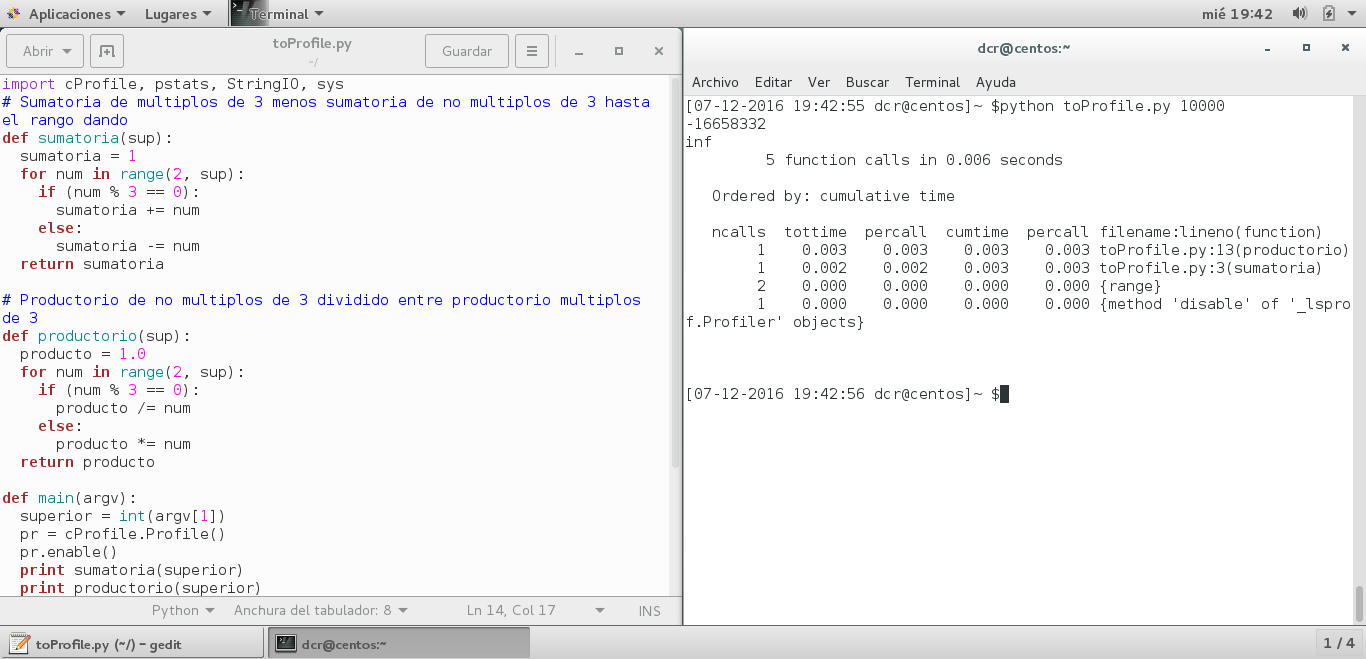
\includegraphics[scale=0.4]{pythonProfile.png}
	\caption{Resultados del profiler cProfile de Python tras ejecutar el script.}
\end{figure}

Podemos observar como el profiler nos devuelve una tabla ordenada por tiempo acumulado de todas las funciones, vemos que la función que más ha tardado ha sido el productorio, seguido inmediatamente de la sumatoria. En la parte superior (antes de la tabla), además de los resultados obtenemos el tiempo total de ejecución y vemos que son 0.006 segundos. En la tabla se nos informa también del número de veces que se llama a una función, el tiempo total y el tiempo acumulado y sus respectivas versiones por llamada a la función. Aunque no hay una diferencia muy grande entre el tiempo de ejecución de la sumatoria y el productorio de los resultados podemos deducir que el cuello de botella de nuestro programa tal y como está es el productorio y si queremos una mejor eficiencia esa es la función que debemos optimizar.

%----------------------------------------------------------------------------------------
%	Cuestión 9
%----------------------------------------------------------------------------------------
\section{Acceda a la consola mysql (o a través de phpMyAdmin) y muestre el resultado de mostrar el ”profile” de una consulta (la creación de la BD y la consulta la puede hacer libremente).}
Vamos a hacerlo a través de phpMyAdmin, primero vamos a crear una base datos y una tabla e insertar una tupla en la misma tal y como podemos apreciar en las siguientes capturas de pantalla. \cite{c9}

\begin{figure}[H]
	\centering
	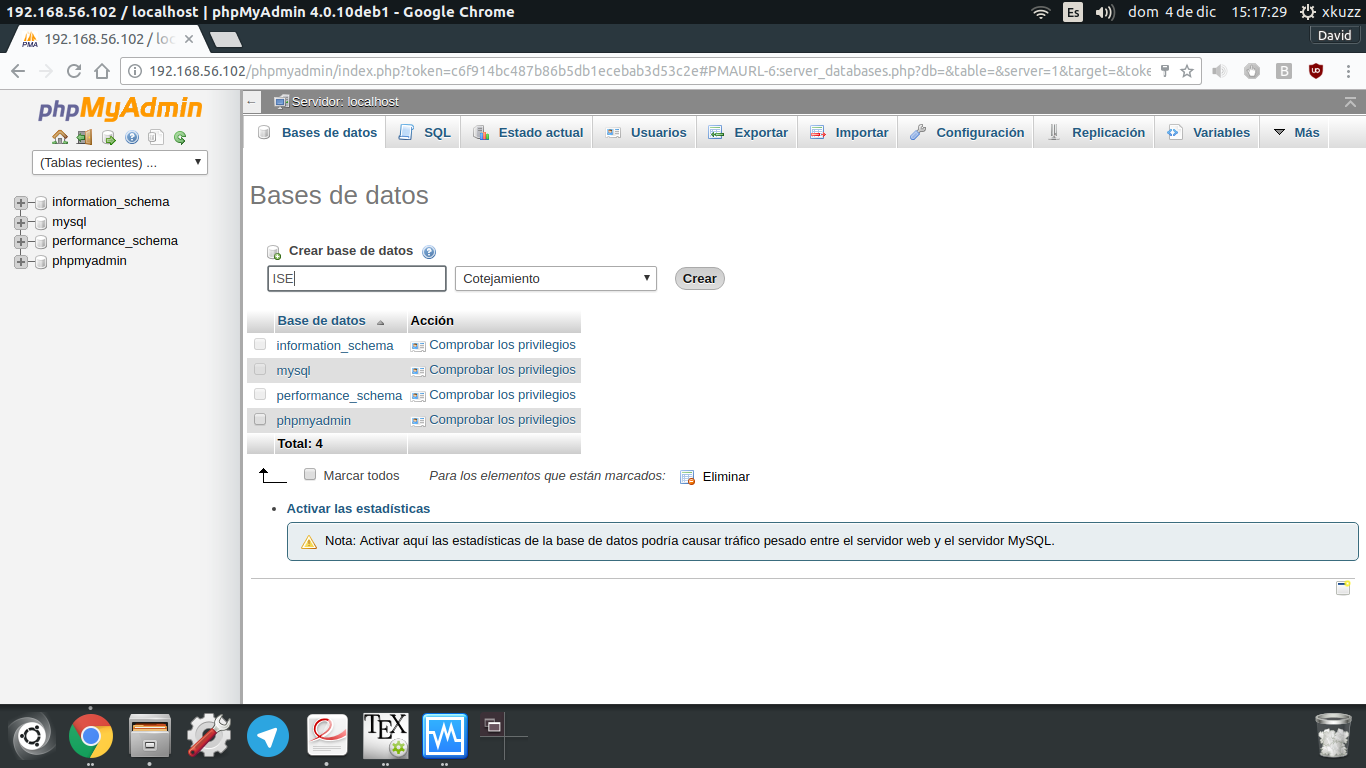
\includegraphics[scale=0.3]{mysql1.png}
	\caption{En \textit{Bases de datos} creamos una nueva base de datos a la que llamamos ISE.}
\end{figure}

\begin{figure}[H]
	\centering
	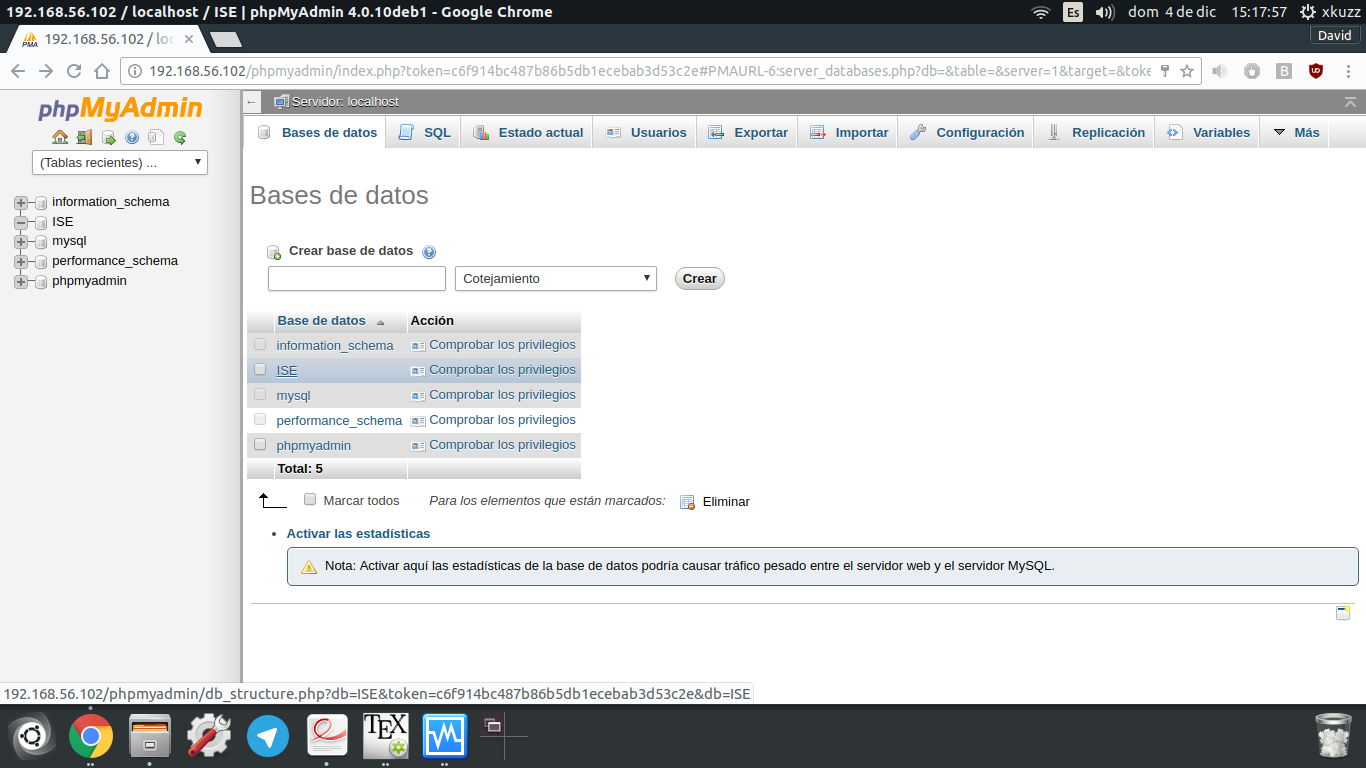
\includegraphics[scale=0.3]{mysql2.png}
	\caption{Pulsamos en la lista de bases de datos \textit{ISE}.}
\end{figure}

\begin{figure}[H]
	\centering
	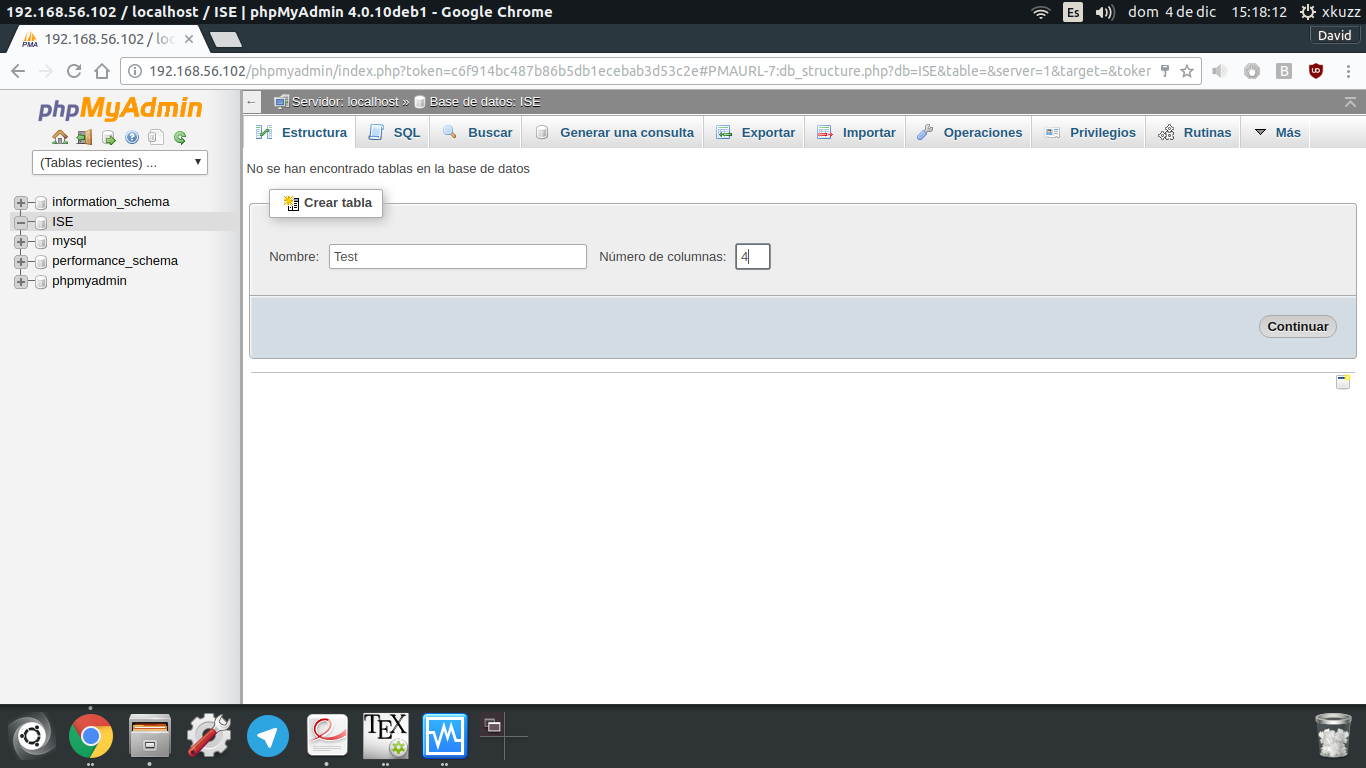
\includegraphics[scale=0.3]{mysql3.png}
	\caption{Creamos una nueva tabla de 4 columnas llamada Test y pulsamos en Enviar.}
\end{figure}

\begin{figure}[H]
	\centering
	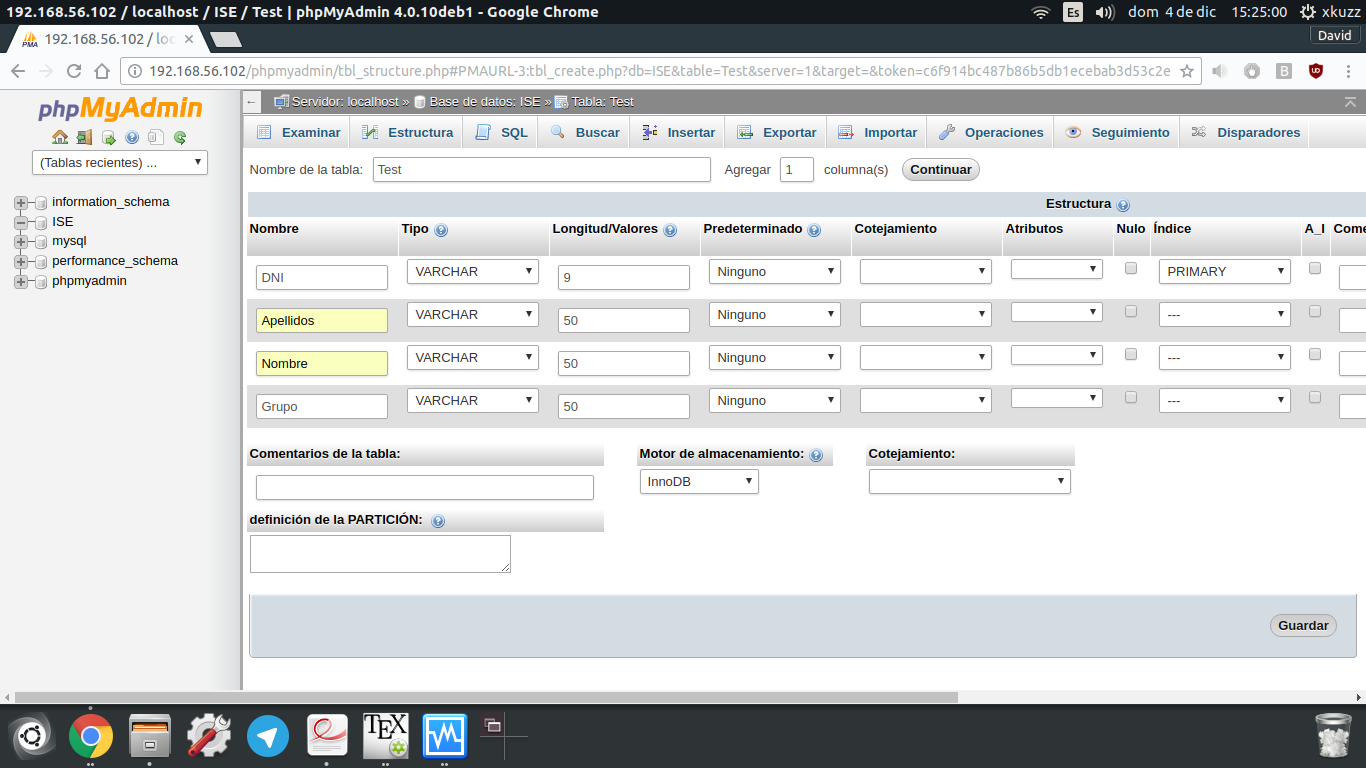
\includegraphics[scale=0.3]{mysql4.png}
	\caption{Creamos una nueva tabla con llave primaria un dni de 9 caracteres y el resto varchar de 50 caracteres (apellidos, nombre, grupo.}
\end{figure}

\begin{figure}[H]
	\centering
	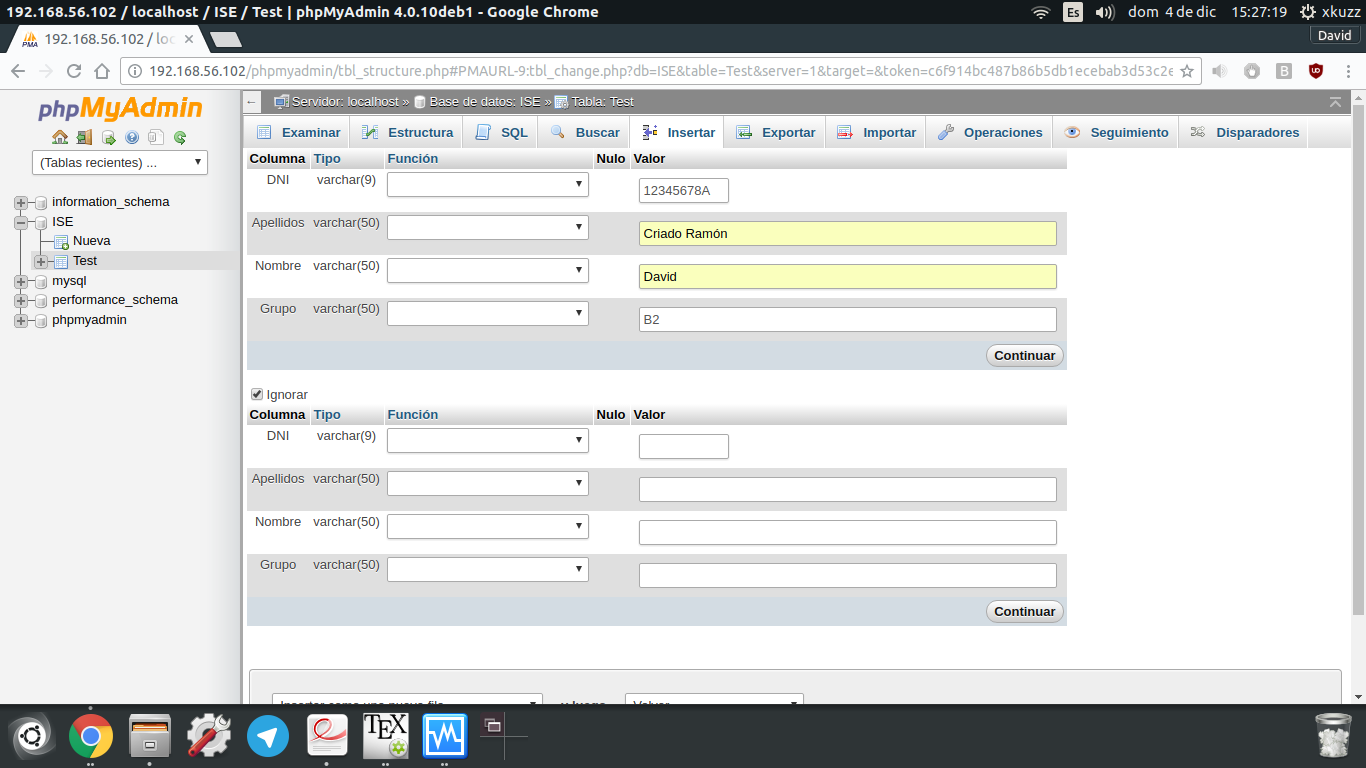
\includegraphics[scale=0.3]{mysql5.png}
	\caption{Insertamos una tupla válida en la tabla pulsando en el menú superior en \textit{Insertar} y rellenando los campos.}
\end{figure}

\begin{figure}[H]
	\centering
	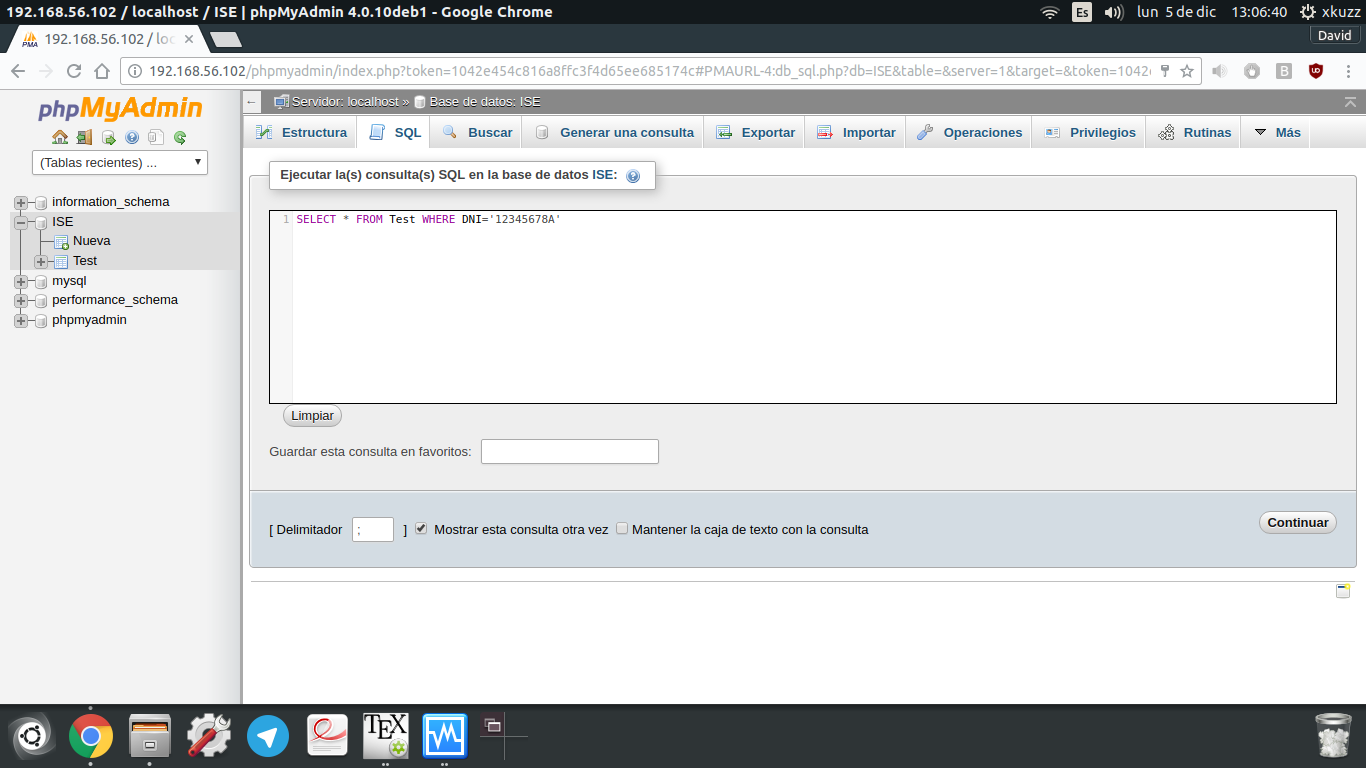
\includegraphics[scale=0.3]{mysqlQuery.png}
	\caption{Pulsamos en la parte superior en SQL y realizamos la consulta. En mi caso he mostrado todos los datos de la tabla de aquellas personas que tuviesen el DNI de la tupla insertada.}
\end{figure}

\begin{figure}[H]
	\centering
	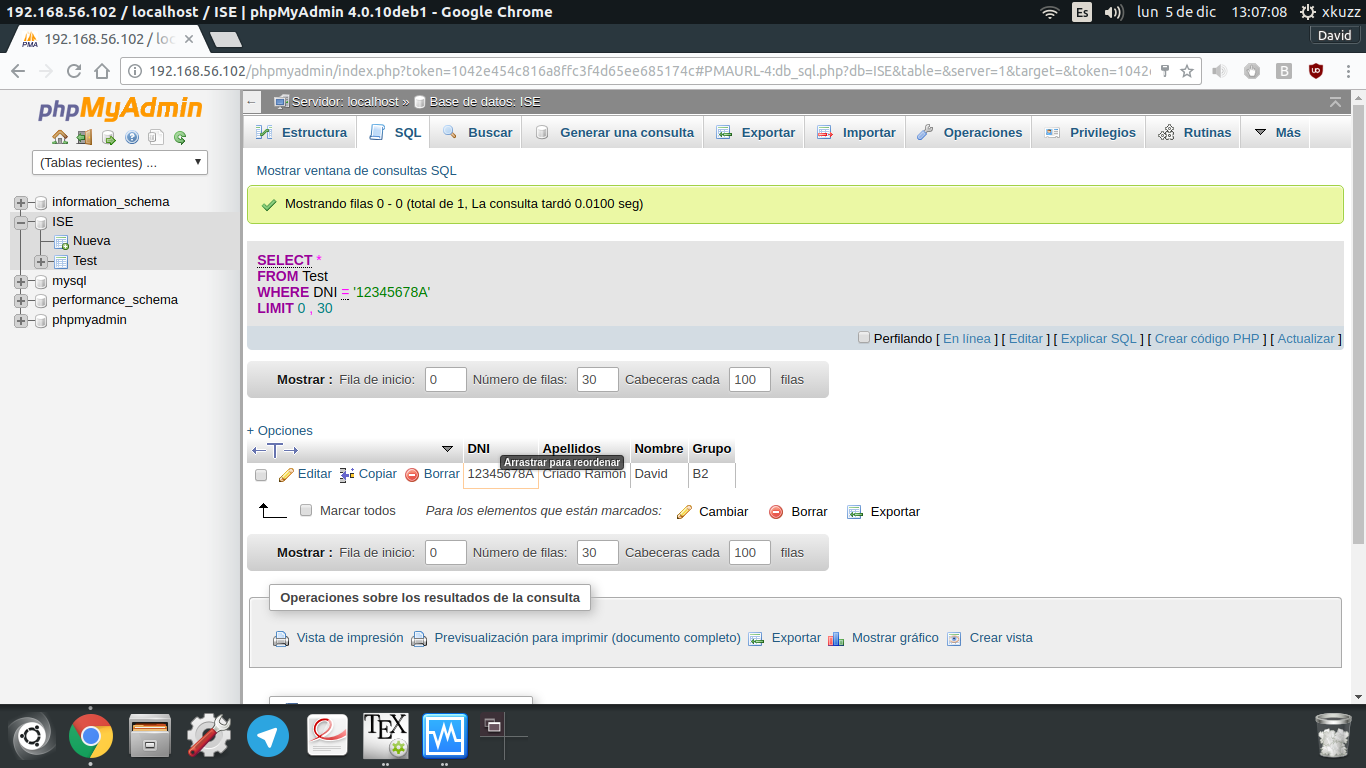
\includegraphics[scale=0.3]{mysqlResult.png}
	\caption{Podemos observar que el único resultado que obtenemos es la tupla que insertamos.}
\end{figure}

\begin{figure}[H]
	\centering
	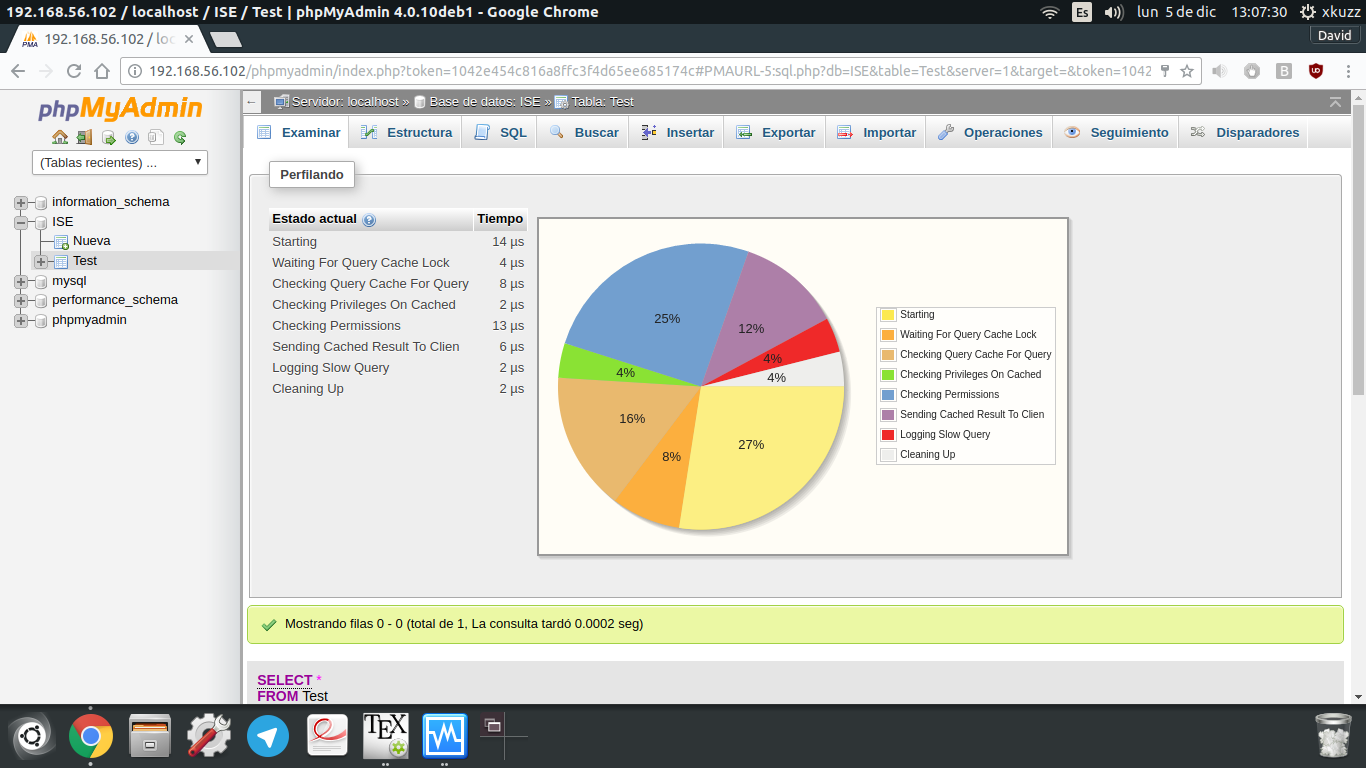
\includegraphics[scale=0.3]{mysqlProfile.png}
	\caption{Tras pulsar en \textit{Perfilando} aparece esta gráfica.}
\end{figure}

A la izquierda podemos observar una tabla en la que viene cada uno de los campos que analiza el \textit{profiler} junto a su tiempo, los cuales se encuentran el rango de los microsegundos. A la derecha tenemos un diagrama de sectores asociados a dichos valores. Podemos observar que debido a la gran sencillez de la consulta la mayor parte del tiempo ha sido dedicada a iniciar y comprobar los permisos. Ambos juntos superan la mitad de los tiempos de la consulta. El siguiente trozo relativamente más grande de tiempo se ha dedicado a comprobar si la consulta estaba en caché y que comprobar los permisos que tenemos en los elementos en caché, registrar la consultar y limpiar han sido las operaciones más rápidas.

%----------------------------------------------------------------------------------------
%	Bibliografía
%----------------------------------------------------------------------------------------
\bibliography{citas} %archivo citas.bib que contiene las entradas 
\bibliographystyle{ieeetr} % hay varias formas de citar
\end{document}
